\documentclass[a4paper,11pt]{article}

\usepackage{fullpage}

\usepackage[utf8]{inputenc}
\usepackage[T1]{fontenc}
\usepackage{graphicx}
\usepackage{float}
\usepackage{hyperref}
\usepackage{url}

\setlength\parindent{0pt}

\usepackage{listings}
\usepackage[usenames,dvipsnames]{color}
\lstset{ 
	language=R,                     % the language of the code
	basicstyle=\scriptsize\ttfamily, % the size of the fonts that are used for the code
	numbers=left,                   % where to put the line-numbers
	numberstyle=\scriptsize\color{Blue},  % the style that is used for the line-numbers
	stepnumber=1,                   % the step between two line-numbers. If it is 1, each line
	% will be numbered
	numbersep=5pt,                  % how far the line-numbers are from the code
	backgroundcolor=\color{white},  % choose the background color. You must add \usepackage{color}
	showspaces=false,               % show spaces adding particular underscores
	showstringspaces=false,         % underline spaces within strings
	showtabs=false,                 % show tabs within strings adding particular underscores
	frame=single,                   % adds a frame around the code
	rulecolor=\color{black},        % if not set, the frame-color may be changed on line-breaks within not-black text (e.g. commens (green here))
	tabsize=2,                      % sets default tabsize to 2 spaces
	captionpos=b,                   % sets the caption-position to bottom
	breaklines=true,                % sets automatic line breaking
	breakatwhitespace=false,        % sets if automatic breaks should only happen at whitespace
	keywordstyle=\color{RoyalBlue},      % keyword style
	commentstyle=\color{Green},     % comment style
	stringstyle=\color{ForestGreen}      % string literal style
} 

\title{Prognose und Probabilistische Budgetierung von künftigen Absatzmengen}

\author{
	KECK Barbara (e1225589) \\
	barbara.keck@gmx.at
	\and
	STRÖMER Stefan (e1225341) \\
	s.stroemer@live.at
}

\date{\today}

\begin{document}

\maketitle

\vskip 5em

\begin{abstract}
	In Ihrer Funktion als Junior-Controller unterstützen Sie die Geschäftsführung bei der Budgetierung. Aufgrund Ihrer Universitätsausbildung bringen Sie die Probabilistische Budgetierung (unter Verwendung von: zeitreihenbasierter Prognose, regressionsbasierter Prognose und Stochastische prozessbasiertre Prognose) ins Unternehmen ein. Dabei werden bei der Prognose und Budgetierung die mit der Zukunft verbundenen Unsicherheiten explizit berücksichtig, womit sich diese Art der Budgetierung deutlich von der üblicherweise eingesetzten Art der Budgetierung unterscheidet, wobei die künftige Unsicherheit weitestgehend vernachlässigt wird.\\
	
	Die von Ihnen zu bewältigenden Aufgaben sind wie folgt:
	\begin{enumerate}
		\item Tägliche Absatzzahlen – Zeitreihenmodell: Erstellen Sie eine rationale Prognose in R für die Absatzmengen des kommenden Jahres bezüglich der gegossenen (A), gepressten (B) und gezogenen Kerzen (C)
		\item Tägliche Absatzzahlen – Regressionsmodellen: Erstellen Sie eine rationale Prognose in R für die Absatzmengen des kommenden Jahres bezüglich der gegossenen (A), gepressten (B) und gezogenen Kerzen (C)
		\item Quartalsweise Absatzzahlen – Stochastische Prozess-Modelle: Erstellen Sie eine rationale Prognose in R für die Absatzmengen des kommenden Jahres bezüglich der Gesamtheit aller Kerzen (ABC) 
		\item Führen Sie eine Literatur-Recherche zum Thema Prognose und Budgetierung durch. Verwenden Sie in Ihren Erläuterungen die in der Literatur gefundenen Prognose- und Budgetierungskonzepte. Zitieren Sie die bei den aus der Literatur verwendeten Konzepten die jeweiligen Quellen gemäß einer aus der Literatur recherchierten Methode. Ergänzen Sie das Literaturverzeichnis um die zusätzlich verwendeten Quellen.
	\end{enumerate}
\end{abstract}

\newpage
\tableofcontents

\newpage
\section{Einführung}

Es liegen Absatz-Daten der letzten beiden Geschäftsjahre vor, basierend auf den Verkäufen dreier unterschiedlicher Arten an Kerzen. Diese Daten enthalten für jeden Verkaufstag (am Wochenende, also Samstag bzw. Sonntag gibt es keinen Verkauf), beginnend mit dem \textbf{01.01.2020} und endend mit dem \textbf{31.12.2021}, die Absatzzahlen unserer drei Kerzenarten (insgesamt 523 Verkaufstage):

\begin{itemize}
	\item Gegossene Kerzen (A)
	\item Gepresste Kerzen (B)
	\item Gezogene Kerzen (C)
\end{itemize}

Bei Durchsicht des Datensatzes fällt zuerst auf, dass abgesehen von den Wochenenden keine Tage fehlen - es wurde auch an Tagen wie dem 24.12. oder dem 01.01. verkauft (und dokumentiert). Wichtig festzuhalten ist jedoch, dass das Jahr 2020 ein Schaltjahr ist (es gibt einen 29.02.2020), das Jahr 2021 nicht (der 28. ist der letzte Tag des Februars). Wir sollten also in unserer Modellierung die Tatsache berücksichtigen, dass Schaltjahre auftreten können.\\

Um einen ersten grundlegenden Überblick über die Daten zu bekommen, betrachten wir einfache Boxplots (dieser zeigt übersichtlich Median und Quartile) sowie den Jahresverlauf der einzelnen Kerzenverkäufe:

\begin{figure}[H]
	\centering
	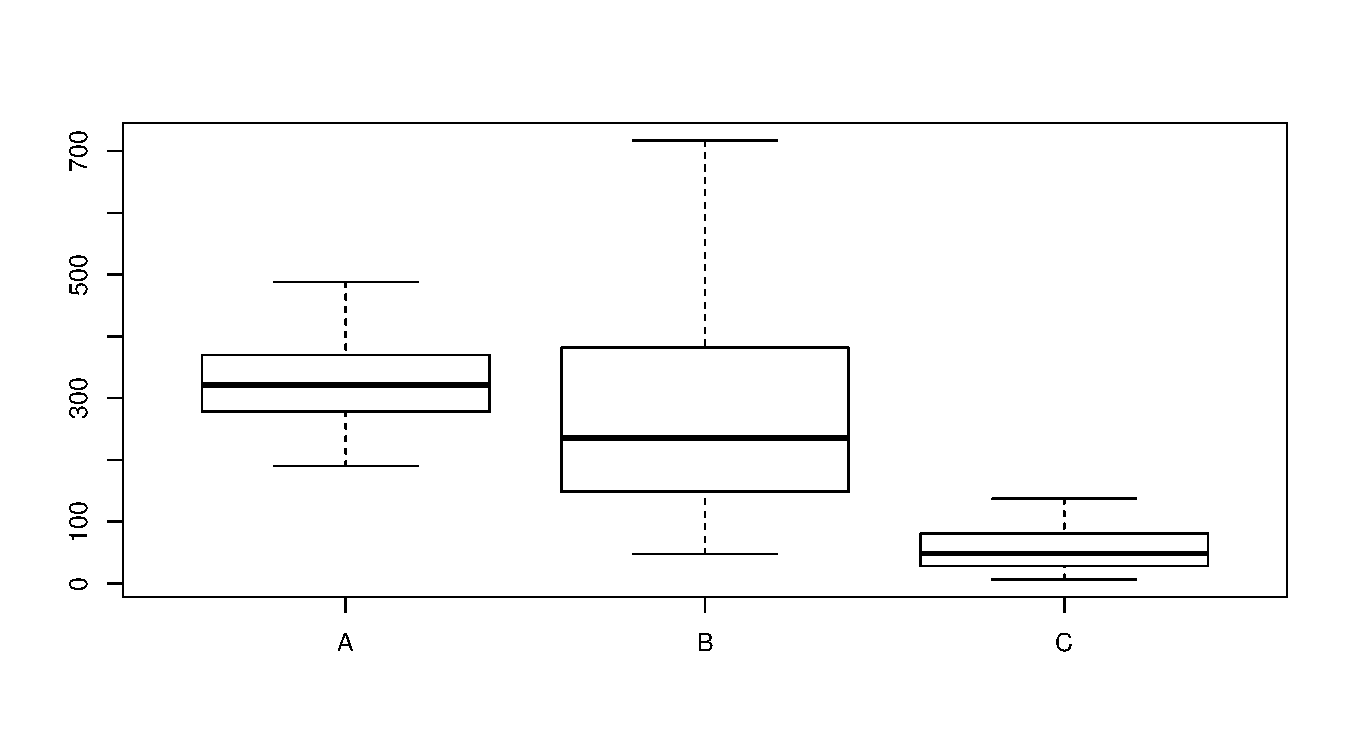
\includegraphics[width=\textwidth]{figures/boxplot.pdf}
	\vskip -1.5em \caption{Boxplot der Kerzen-Absätze}
	\label{fig_boxplot}
\end{figure}

\begin{figure}[H]
	\centering
	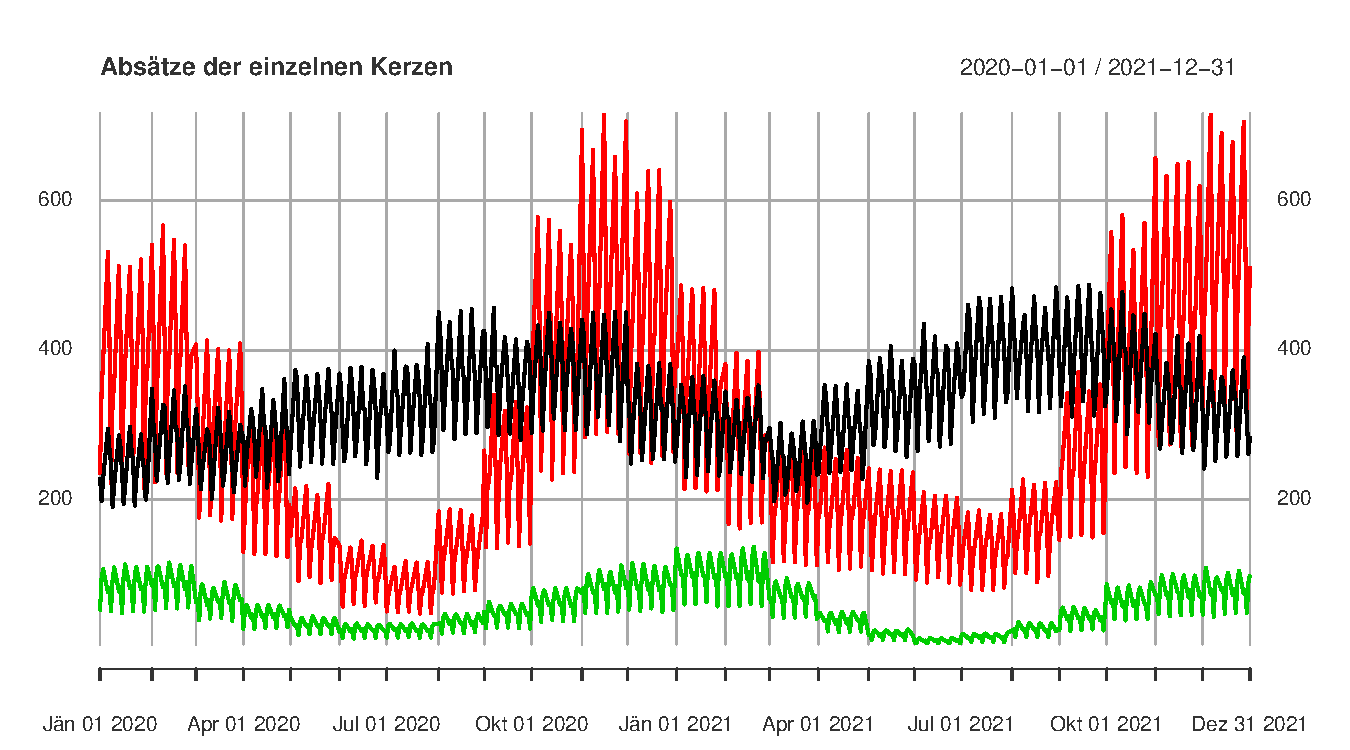
\includegraphics[width=\textwidth]{figures/overview.pdf}
	\vskip -1.5em \caption{Jahresverlauf der Kerzen-Absätze}
	\label{fig_overview}
\end{figure}

\vskip 3em

Wir sehen hier bereits deutliche Unterschiede an absoluten Absatzzahlen. Kerzentyp B scheint außerdem deutlich volatiler (über das gesamte Jahr betrachtet) zu sein, als die beiden anderen Typen.

Schlussendlich bleibt noch festzuhalten wie wir die fehlenden Wochenenden berücksichtigen werden: Gerade für zeitreihenbasierte Vorhersagen ist es wichtig, dies korrekt zu behandeln, da sonst eventuell keine korrekten Saisonalitäten festlegbar sind. Wir halten zuerst fest (manuell observiert aufgrund der Daten):

\begin{itemize}
	\item Eine Woche (7 Tage) besteht aus 5 Einträgen (Montag-Freitag).
	\item Eine gängige / häufig benutzte Konvention zur Berücksichtigung von Schaltjahren ist es, die Jahresperiode mit 365.25 Tagen anzusetzen. Dies ergibt nach vier Jahren (die auf jeden Fall ein Schaltjahr inkludieren) wieder einen Tageszyklus von 1461 Tagen.
\end{itemize}

Unter Berücksichtigung der beiden genannten Punkte ergibt sich somit:

\begin{itemize}
	\item Ein Monat hat eine "Dauer" von $\frac{365.25}{12} \cdot \frac{5}{7}$ Tagen (ungefähr 22).
	\item Ein Quartal hat eine "Dauer" von $\frac{365.25}{4} \cdot \frac{5}{7}$ Tagen (ungefähr 65).
	\item Ein Jahr hat eine "Dauer" von $365.25 \cdot \frac{5}{7}$ Tagen (ungefähr 261).
\end{itemize}

\newpage
Betrachten wir die Auto- bzw. Kreuzkorrelationen (siehe \ref{fig_acf}) der einzelnen Kerzen, so sehen wir geringfügige Korrelationen sogar zwischen den einzelnen Kerzen-Typen. Am stärksten sticht jedoch die Korrelation mit den Vielfachen des Tages-Lags=5 heraus, was unsere manuelle Observation untermauert.

\begin{figure}[H]
	\centering
	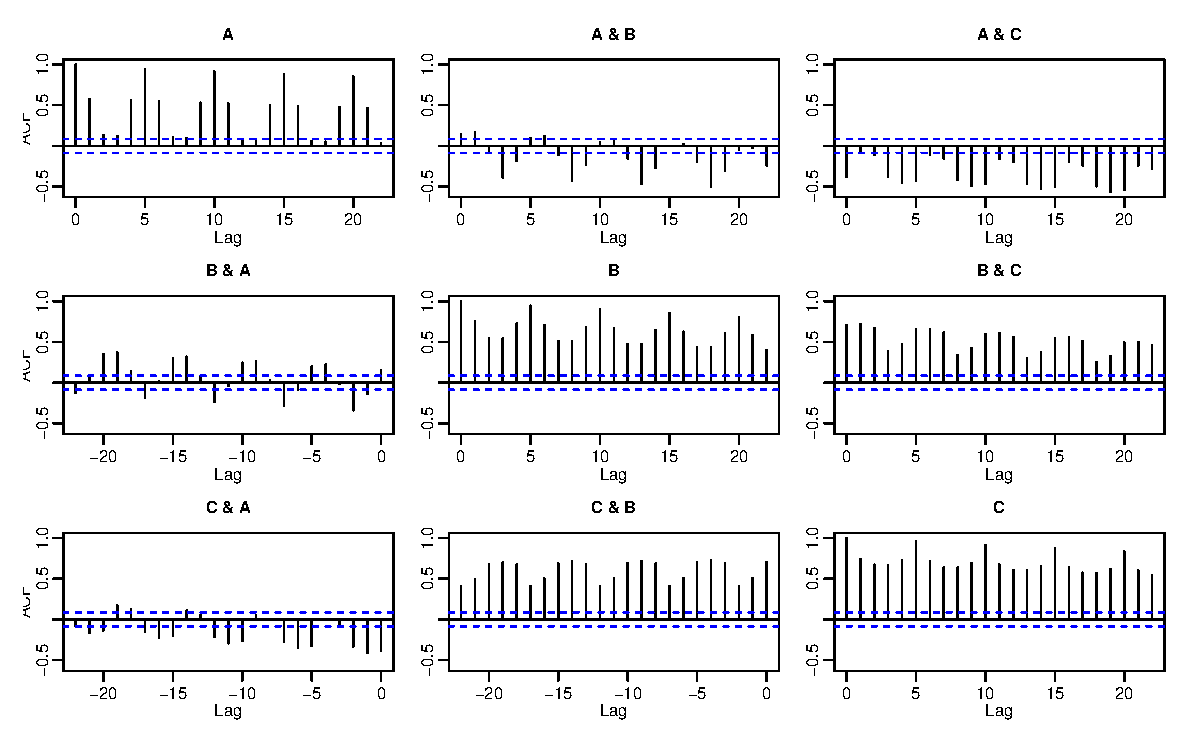
\includegraphics[width=\textwidth]{figures/acf.pdf}
	\vskip -1.5em \caption{ACF / CCF der Kerzen-Absätze}
	\label{fig_acf}
\end{figure}


\newpage
\section{Tägliche Absatzzahlen: Zeitreihenbasierte Budgetierung}

\subsection{Beschreibung der Vorgehensweise}
Eine wichtige Grundlage bei der zeitreihenbasierten Vorhersage mittels sogenannten "timeseries" in R ist die korrekte Erstellung. Hier ist besonders auf den "frequency" Parameter zu achten, der spezifiziert wie viele Observationen pro gegebener Zeiteinheit geliefert werden. Neben der "offensichtlichen" (und beobachteten) Korrelation mit Lag 5 (Mittwochs-Verkäufe ähneln vorangegangenen Mittwochs-Verkäufen) ist besonders der Jahres-Lag wichtig zu beachten. Dieser beschreibt die Eigenschaft, dass Verkäufe zu ähnlichen Jahreszeiten (Weihnachten, Sommer, ...) stark korreliert sind. \\

Wir verwenden für einen ersten Einblick die allgemeine Vorhersage Funktion des Paktes "forecast" \cite{forecast}. Diese benutzt für die Vorhersage eine Kombination aus STL \cite{stl} (Seasonal, Trend, Irregular mittels Loess) und ein ETS \cite{ets} (= Error, Trend, Seasonal) Modell. 

\subsection{Mathematische Beschreibung der verwendeten Prognosemodelle}
\subsection{Erläuterung der Ergebnisse für gegossene, gezogene und gepresste Kerzen}

Die folgenden drei Abbildungen zeigen den prognostizierten Verlauf der Absätze im kommenden Jahr - aufgeteilt nach Kerzentypen. In Grau bzw. Dunkel-Grau werden die 95\% bzw. 80\% Konfidenzintervalle dargestellt. Wir sehen Verläufe die "optisch" einer Kombination der beiden vorangegangenen Jahre entsprechen. Großer Vorteil dieser tageweisen Vorhersage ist, dass sie prinzipiell am Ende jedes Tages neu berechnet werden kann (nun mit mehr Daten) und eine genauere Prognose für den kommenden Zeitraum liefert (dies kann zum Beispiel benutzt werden, um rolling-window Vorhersagen der erwarteten Absätze der jeweils nächsten fünf Tage durchzuführen).\\

Wir erwarten (gerundete) Tagesabsätze im Bereich:
\begin{itemize}
	\item A $\in [220,485]$
	\item B $\in [120,735]$
	\item C $\in [0,120]$
	\item A+B+C  $\in [340,1340]$
\end{itemize}

\begin{figure}[H]
	\centering
	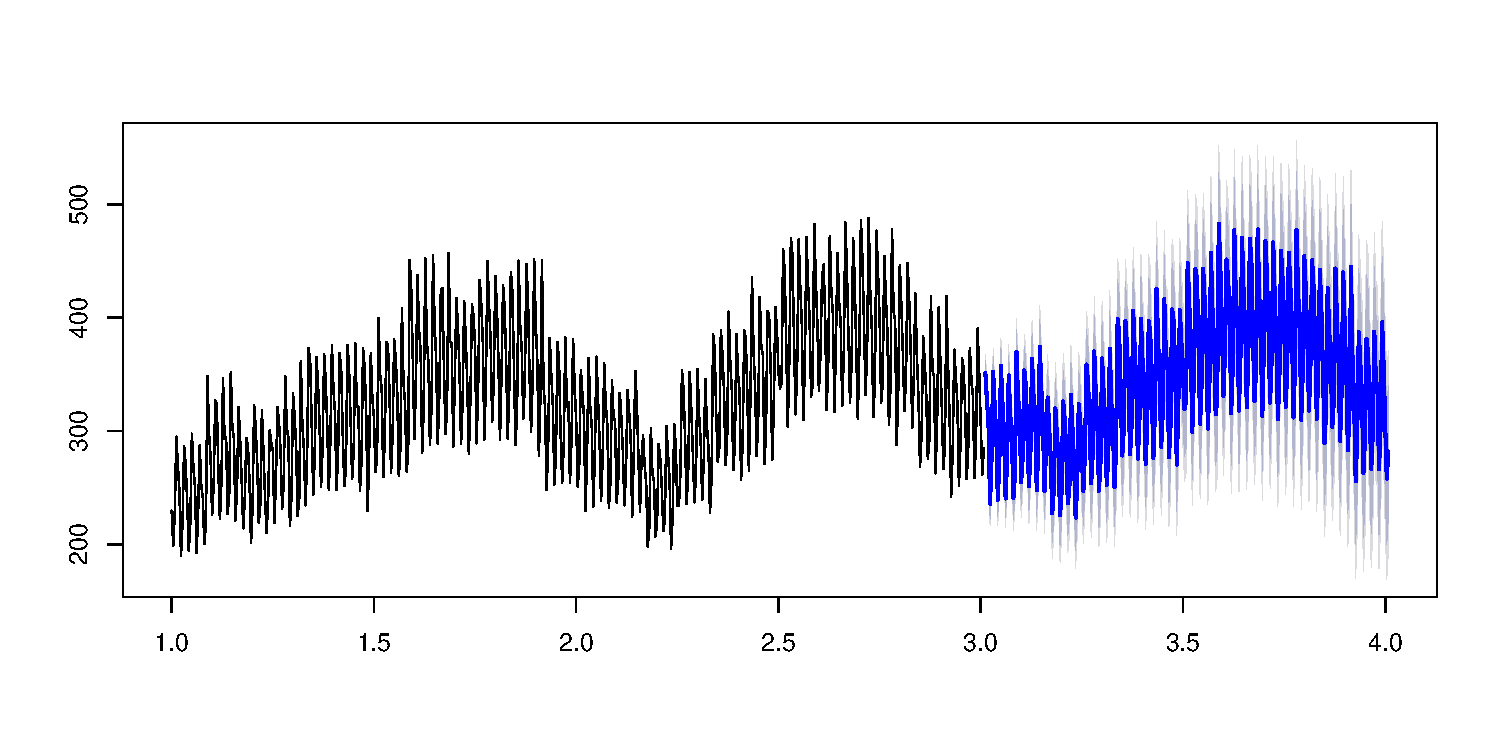
\includegraphics[width=\textwidth]{figures/fc_auto_A.pdf}
	\vskip -1.5em \caption{Zeitreihen - Tagesprognose - Kerzentyp A}
	\label{fig_auto_A}
\end{figure}

\begin{figure}[H]
	\centering
	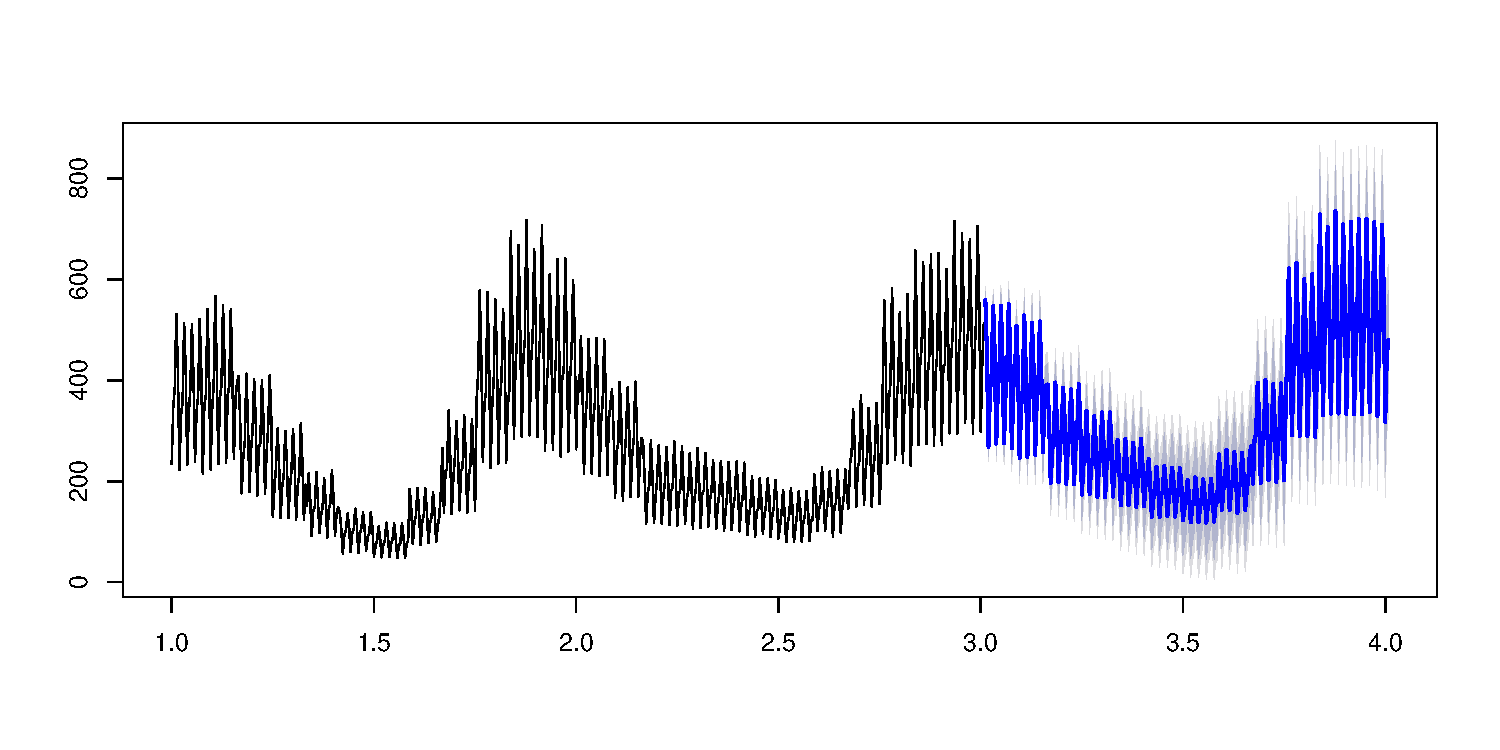
\includegraphics[width=\textwidth]{figures/fc_auto_B.pdf}
	\vskip -1.5em \caption{Zeitreihen - Tagesprognose - Kerzentyp B}
	\label{fig_auto_B}
\end{figure}

\begin{figure}[H]
	\centering
	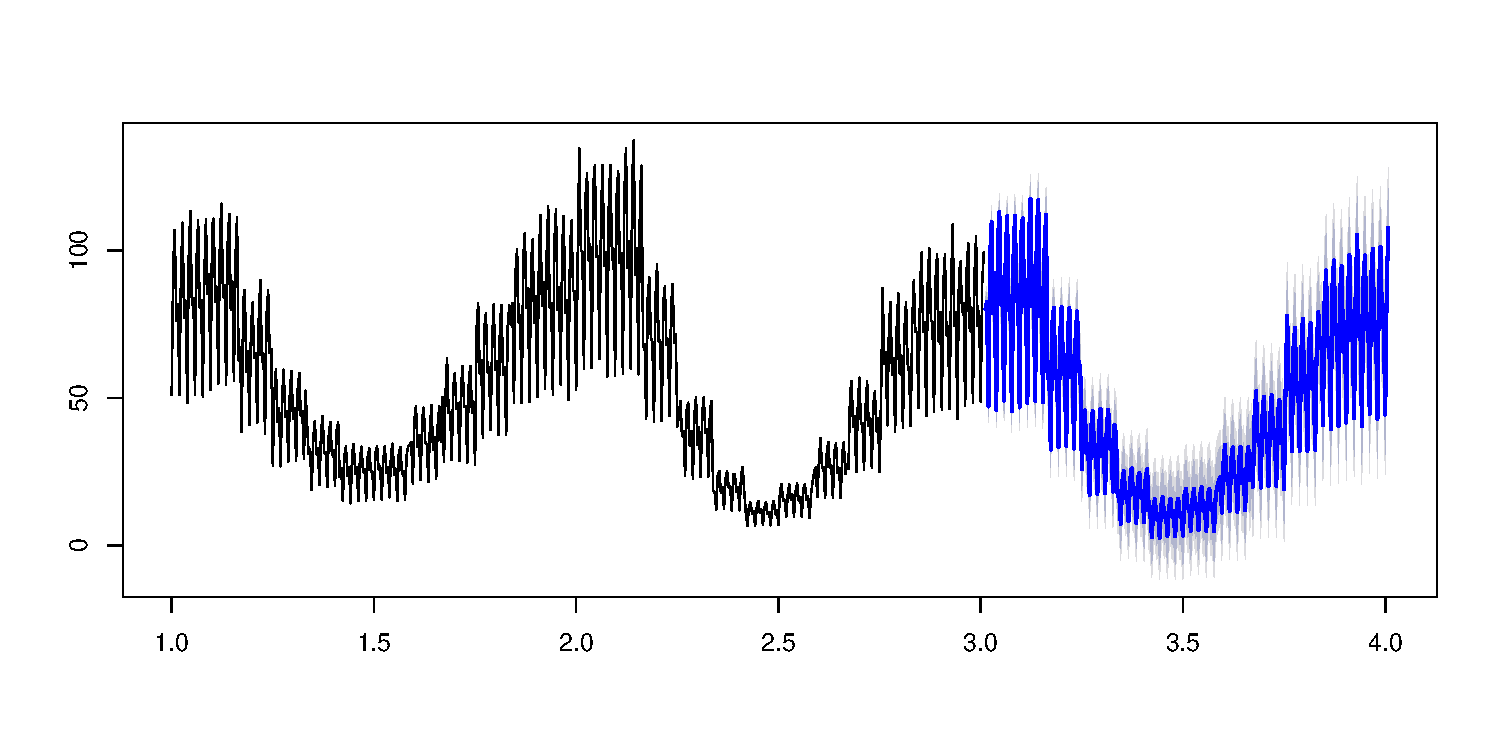
\includegraphics[width=\textwidth]{figures/fc_auto_C.pdf}
	\vskip -1.5em \caption{Zeitreihen - Tagesprognose - Kerzentyp C}
	\label{fig_auto_C}
\end{figure}

\newpage
Die kumulierten Absätze ergeben uns einen "Fahrplan" der einzelnen Jahresabsätze der Produkte für das kommende Jahr.

\begin{figure}[H]
	\centering
	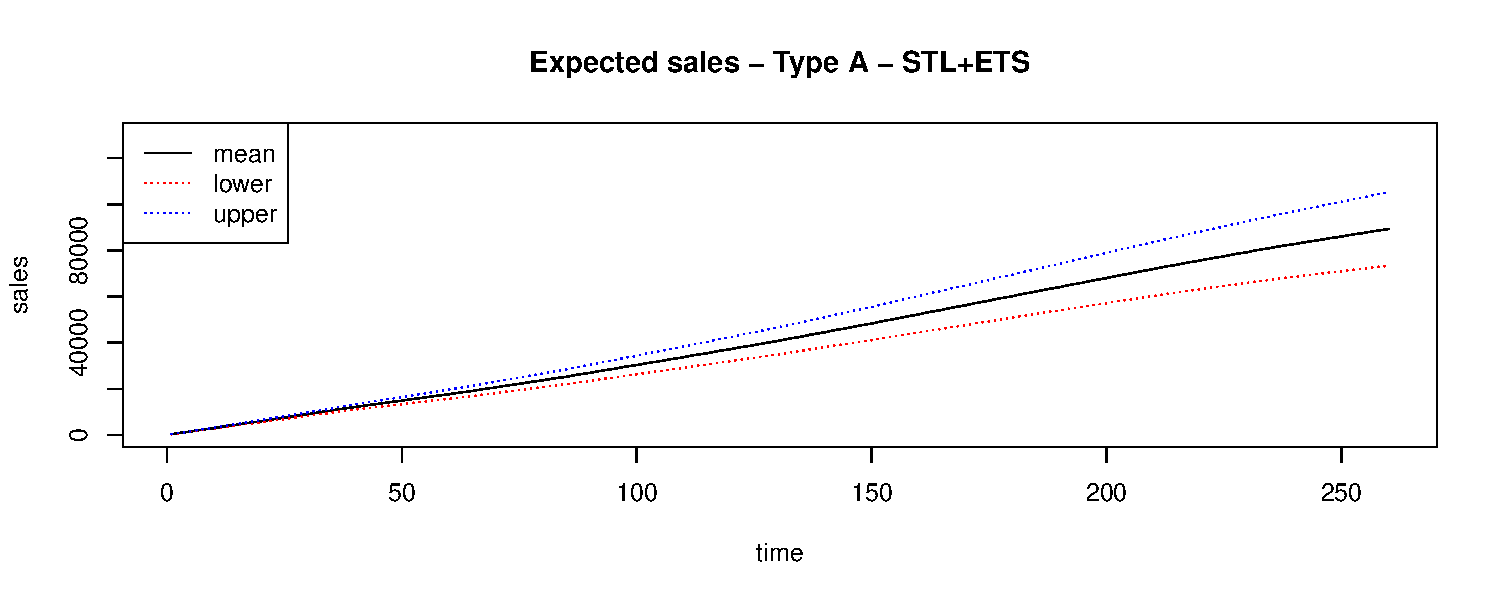
\includegraphics[width=\textwidth]{figures/traj_auto_A.pdf}
	\vskip -1.5em \caption{Zeitreihen - Jahresprognose - Kerzentyp A}
	\label{traj_auto_A}
\end{figure}
\begin{figure}[H]
	\centering
	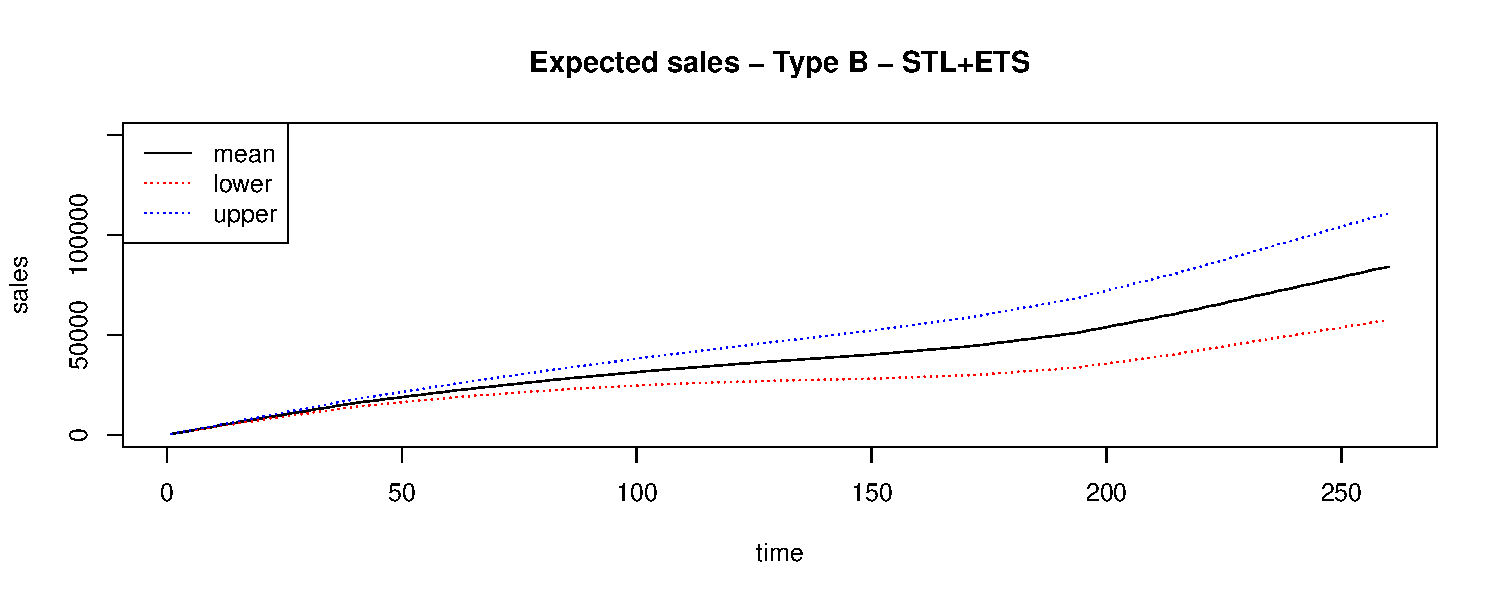
\includegraphics[width=\textwidth]{figures/traj_auto_B.pdf}
	\vskip -1.5em \caption{Zeitreihen - Jahresprognose - Kerzentyp B}
	\label{traj_auto_B}
\end{figure}
\begin{figure}[H]
	\centering
	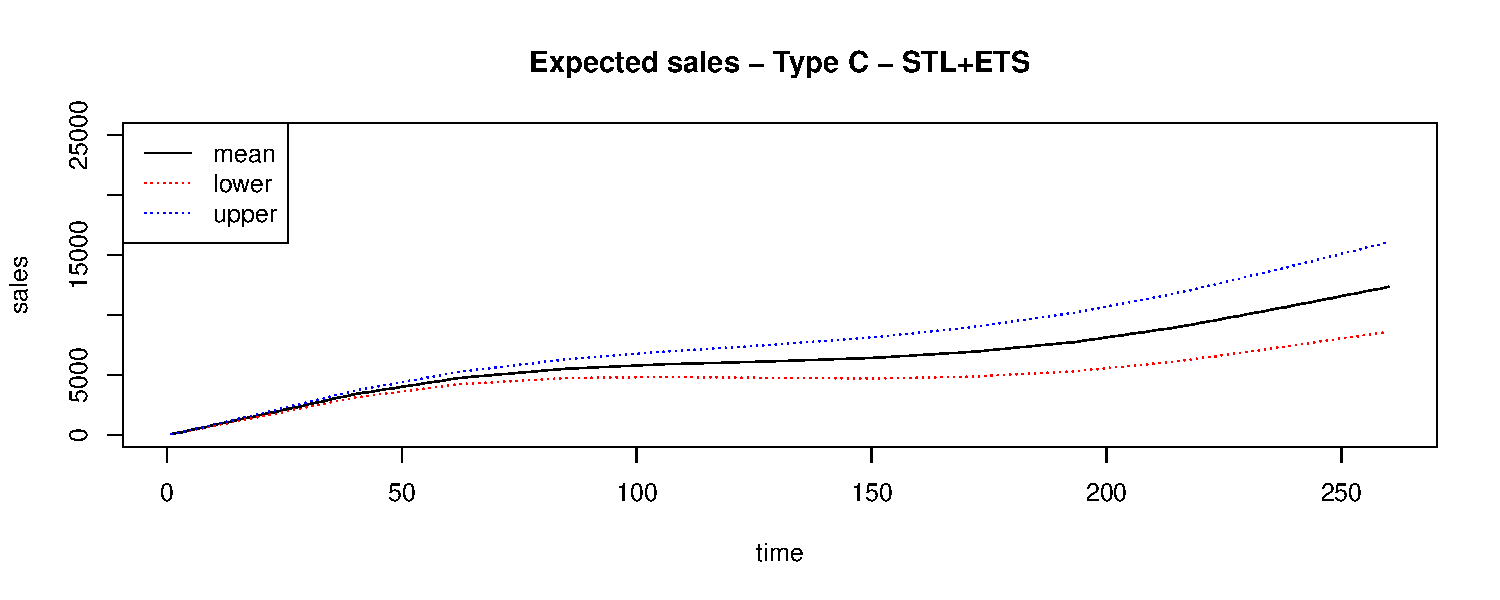
\includegraphics[width=\textwidth]{figures/traj_auto_C.pdf}
	\vskip -1.5em \caption{Zeitreihen - Jahresprognose - Kerzentyp C}
	\label{traj_auto_C}
\end{figure}


\subsection{Angabe des R-Codes mit Erläuterungen}

\begin{lstlisting}
# Specify one seasonality manually:
# 365.25 days per year on average (accounting for leap-years)
# 7 days a week normally
# 5 days a week in our dataset (since we skip weekends)

# Do an automated forecast (this uses STL and ETS)
forecast.ts.auto <- forecast(candles.ts, 365.25/7*5)

# Plot the basic forecasts
plot(forecast.ts.auto$forecast$A, main="")
plot(forecast.ts.auto$forecast$B, main="")
plot(forecast.ts.auto$forecast$C, main="")

# Convert them into dataframes for better plotting
forecast.ts.auto.agg.A <- forecast2dataframe(forecast.ts.auto$forecast$A, TRUE)
forecast.ts.auto.agg.B <- forecast2dataframe(forecast.ts.auto$forecast$B, TRUE)
forecast.ts.auto.agg.C <- forecast2dataframe(forecast.ts.auto$forecast$C, TRUE)

# Plot the trajectories through the predicted year
cumsumplot(forecast.ts.auto.agg.A, "Expected sales - Type A - STL+ETS", scale.A)
cumsumplot(forecast.ts.auto.agg.B, "Expected sales - Type B - STL+ETS", scale.B)
cumsumplot(forecast.ts.auto.agg.C, "Expected sales - Type C - STL+ETS", scale.C)

# Plot the accumulated trajectory through the year (all candle sales)
ccumsumplot(forecast.ts.auto.agg.A, forecast.ts.auto.agg.B, forecast.ts.auto.agg.C,
            "Expected sales - All candles - STL+ETS", scale.ABC)
\end{lstlisting}

\newpage
\section{Tägliche Absatzzahlen: Regressionsbasierte Budgetierung}

\subsection{Beschreibung der Vorgehensweise}

Um eine geeignete Regression durchführen zu können, müssen wir zunächst konkrete erklärende Variablen erzeugen - die reine Regression auf den Tagesindex würde zu wenig Erfolg führen. Wir generieren deshalb zusätzliche Daten, die das Quartal, das Monat sowie den Wochentag eines Datensatzes beschreiben. Zwei weitere (Tag des Monats sowie Index der Woche im Jahr) wurden testweise aufgenommen, jedoch aufgrund von fehlender statistischer Signifikanz wieder verworfen.\\

Die Faktorisierung von erklärenden Variablen erleichtert uns die Beschreibung und Darstellung von nicht-linearen Zusammenhängen. So beschreiben beispielsweise die Wochentage eine beinahe perfekte Gerade mit den Einflüssen $0, -33, -66, -97, -130$ - jedoch in verkehrter Reihenfolge $1, 2, 3, 5, 4$. Diese Daten durch eine Gerade zu approximieren würde einen starken Fehler in unserer Prognose verursachen. Aufgrund der Faktorisierung können wir jedem Wochentag einen eigenen geschätzten Parameter zuweisen.\\

Anmerkung: Ein hinzufügen eines "Kreuzterm" wie "year*as.factor(month)" löst eines der "offensichtlicheren" Probleme der Regression: Wir erwarten uns Residuen die als weißes Rauschen um Null verteilt sind. Dies ist offensichtlich nicht (ganz) der Fall - eine Abhängigkeit vom Zeitindex ist immer noch zu sehen. Allerdings ist diese Abhängigkeit nicht periodisch erklärbar, wodurch eine Erklärung durch individuelle Monatsterme auf jeden Fall \textbf{nur} zu einem Overfitting führt und die Prognosequalität reduziert. Wir akzeptieren daher im Moment die "nicht idealen" Residuen um die Prognosequalität nicht künstlich zu verschlechtern - sollte eine komplexere Vorhersage/Unternehmensentscheidung auf diesen Resultaten aufbauen, müsste dieser "Fehler" noch behoben oder zumindest genauer untersucht werden.\\

Ein zu untersuchender Faktor der hier eine Rolle spielen (kann) sind nicht zeitlich fixierte Feiertage (z.B. Ostern). Diese können durchaus auch in die Untersuchung miteinbezogen werden - dies würden den Rahmen der vorliegenden Arbeit aber sprengen. Siehe dazu unter anderem \cite{holidays} von Rob J. Hyndman.

\subsection{Mathematische Beschreibung der verwendeten Prognosemodelle}
\subsection{Erläuterung der Ergebnisse für gegossene, gezogene und gepresste Kerzen}

\newpage
Zuerst betrachten wir die Residuen grafisch:

\begin{figure}[H]
	\centering
	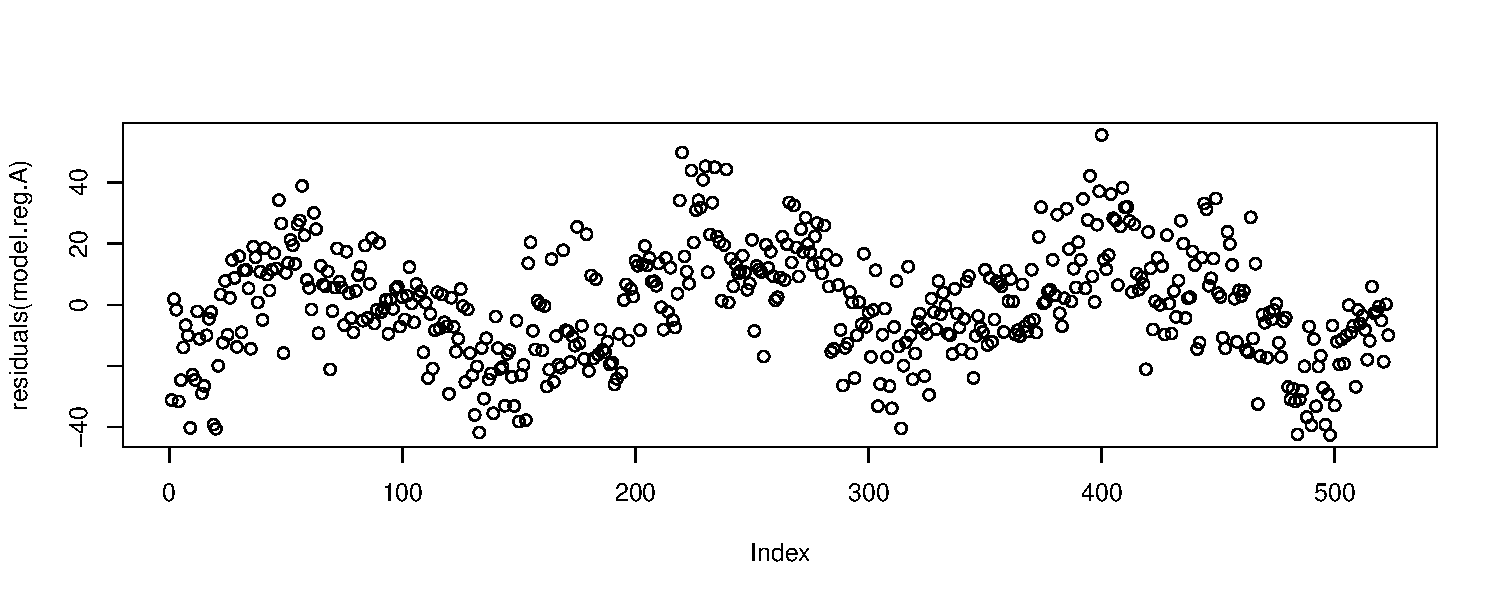
\includegraphics[width=\textwidth]{figures/res_reg_A.pdf}
	\vskip -1.5em \caption{Regression - Residuen - Kerzentyp A}
	\label{fig_res_A}
\end{figure}

\begin{figure}[H]
	\centering
	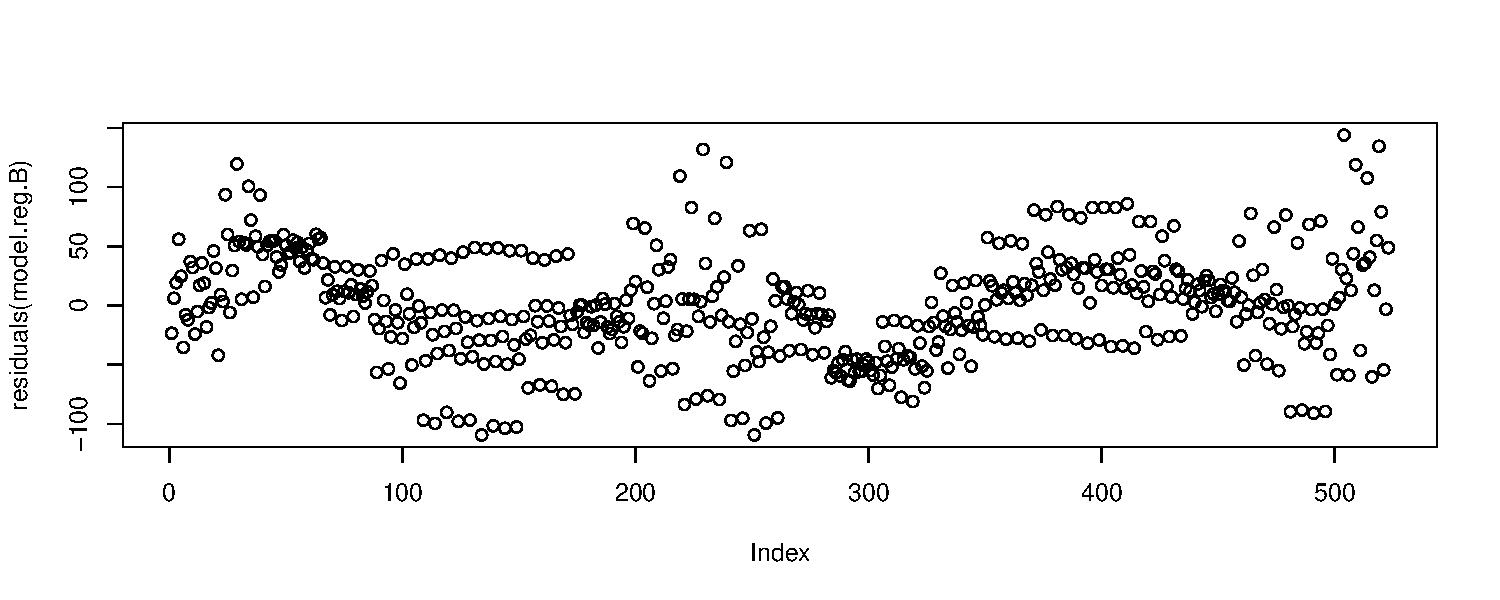
\includegraphics[width=\textwidth]{figures/res_reg_B.pdf}
	\vskip -1.5em \caption{Regression - Residuen - Kerzentyp B}
	\label{fig_res_B}
\end{figure}

\begin{figure}[H]
	\centering
	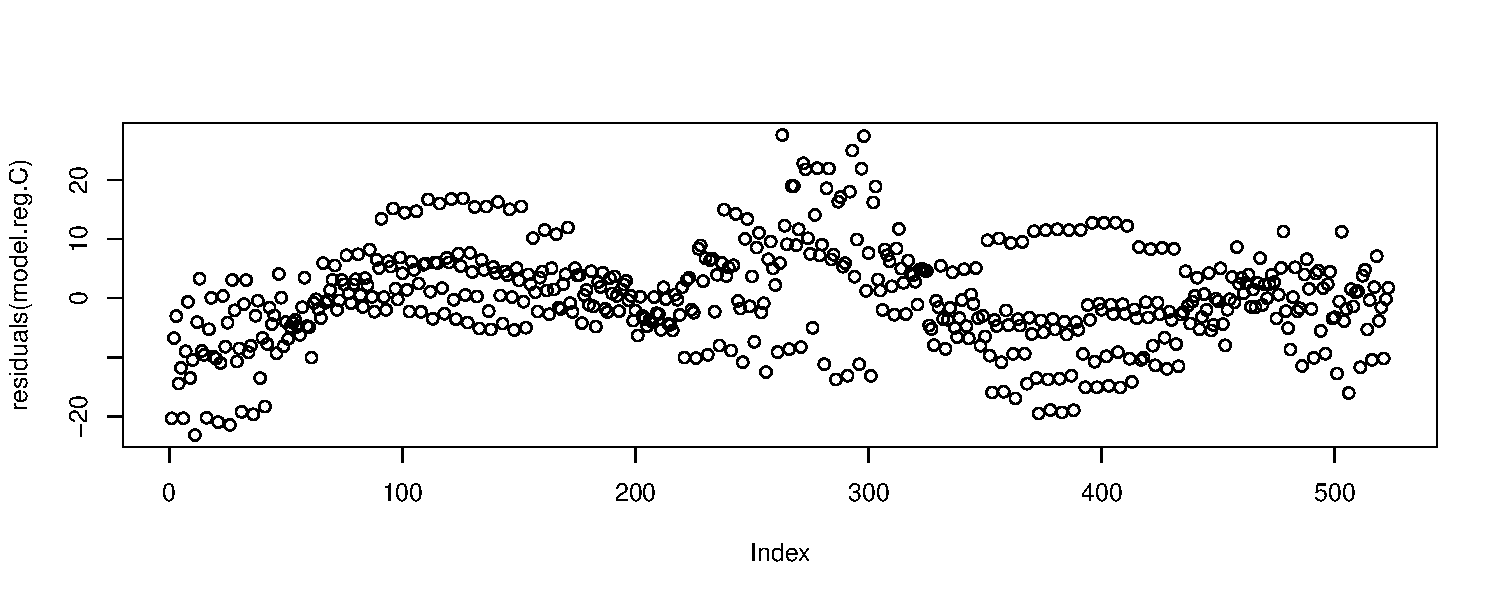
\includegraphics[width=\textwidth]{figures/res_reg_C.pdf}
	\vskip -1.5em \caption{Regression - Residuen - Kerzentyp C}
	\label{fig_res_C}
\end{figure}

\newpage
Ein Blick auf die summary der einzelnen Kerzentypen:

%\lstinputlisting{figures/summary.txt}
\begin{lstlisting}
Call:
lm(formula = A ~ year + as.factor(quarter) + as.factor(month) + 
as.factor(dayOfWeek), data = candles.xts)

Residuals:
Min      1Q  Median      3Q     Max 
-42.583 -11.729   0.389  11.829  55.528 

Coefficients: (3 not defined because of singularities)
Estimate Std. Error t value Pr(>|t|)    
(Intercept)            307.331      3.964  77.538  < 2e-16 ***
year                    19.226      1.591  12.085  < 2e-16 ***
as.factor(quarter)2     57.827      3.880  14.904  < 2e-16 ***
as.factor(quarter)3    107.298      3.879  27.661  < 2e-16 ***
as.factor(quarter)4     45.259      3.836  11.798  < 2e-16 ***
as.factor(month)2       14.325      3.974   3.605 0.000344 ***
as.factor(month)3      -16.831      3.859  -4.361 1.57e-05 ***
as.factor(month)4      -41.964      3.880 -10.816  < 2e-16 ***
as.factor(month)5       -9.488      3.925  -2.418 0.015977 *  
as.factor(month)6           NA         NA      NA       NA    
as.factor(month)7      -20.169      3.857  -5.229 2.50e-07 ***
as.factor(month)8        3.399      3.902   0.871 0.384129    
as.factor(month)9           NA         NA      NA       NA    
as.factor(month)10      58.843      3.859  15.248  < 2e-16 ***
as.factor(month)11      34.656      3.860   8.977  < 2e-16 ***
as.factor(month)12          NA         NA      NA       NA    
as.factor(dayOfWeek)2  -33.141      2.523 -13.136  < 2e-16 ***
as.factor(dayOfWeek)3  -65.810      2.519 -26.125  < 2e-16 ***
as.factor(dayOfWeek)4 -129.798      2.520 -51.505  < 2e-16 ***
as.factor(dayOfWeek)5  -96.546      2.520 -38.314  < 2e-16 ***
---
Signif. codes:  0 '***' 0.001 '**' 0.01 '*' 0.05 '.' 0.1 ' ' 1

Residual standard error: 18.19 on 506 degrees of freedom
Multiple R-squared:  0.9254,	Adjusted R-squared:  0.923 
F-statistic: 392.1 on 16 and 506 DF,  p-value: < 2.2e-16
\end{lstlisting}
\begin{lstlisting}
Call:
lm(formula = B ~ year + as.factor(quarter) + as.factor(month) + 
as.factor(dayOfWeek), data = candles.xts)

Residuals:
Min       1Q   Median       3Q      Max 
-109.339  -27.957    0.389   30.178  143.964 

Coefficients: (3 not defined because of singularities)
Estimate Std. Error t value Pr(>|t|)    
(Intercept)            480.377      9.687  49.587  < 2e-16 ***
year                    -4.933      3.888  -1.269 0.205130    
as.factor(quarter)2   -239.799      9.483 -25.288  < 2e-16 ***
as.factor(quarter)3   -120.700      9.481 -12.731  < 2e-16 ***
as.factor(quarter)4    100.953      9.376  10.768  < 2e-16 ***
as.factor(month)2      -28.091      9.713  -2.892 0.003991 ** 
as.factor(month)3     -122.315      9.432 -12.968  < 2e-16 ***
as.factor(month)4       76.658      9.482   8.084 4.64e-15 ***
as.factor(month)5       35.962      9.592   3.749 0.000198 ***
as.factor(month)6           NA         NA      NA       NA    
as.factor(month)7     -135.050      9.428 -14.324  < 2e-16 ***
as.factor(month)8     -100.787      9.537 -10.568  < 2e-16 ***
as.factor(month)9           NA         NA      NA       NA    
as.factor(month)10     -67.632      9.432  -7.171 2.67e-12 ***
as.factor(month)11       8.839      9.435   0.937 0.349322    
as.factor(month)12          NA         NA      NA       NA    
as.factor(dayOfWeek)2  -83.658      6.166 -13.567  < 2e-16 ***
as.factor(dayOfWeek)3 -218.134      6.157 -35.430  < 2e-16 ***
as.factor(dayOfWeek)4 -135.806      6.159 -22.049  < 2e-16 ***
as.factor(dayOfWeek)5 -108.345      6.159 -17.592  < 2e-16 ***
---
Signif. codes:  0 '***' 0.001 '**' 0.01 '*' 0.05 '.' 0.1 ' ' 1

Residual standard error: 44.45 on 506 degrees of freedom
Multiple R-squared:  0.9165,	Adjusted R-squared:  0.9138 
F-statistic: 346.9 on 16 and 506 DF,  p-value: < 2.2e-16
\end{lstlisting}
\begin{lstlisting}
Call:
lm(formula = C ~ year + as.factor(quarter) + as.factor(month) + 
as.factor(dayOfWeek), data = candles.xts)

Residuals:
Min       1Q   Median       3Q      Max 
-23.1253  -4.5344  -0.3595   4.7874  27.5802 

Coefficients: (3 not defined because of singularities)
Estimate Std. Error t value Pr(>|t|)    
(Intercept)            93.5979     1.8292  51.168  < 2e-16 ***
year                   -2.9769     0.7342  -4.054 5.82e-05 ***
as.factor(quarter)2   -73.0239     1.7906 -40.782  < 2e-16 ***
as.factor(quarter)3   -46.9761     1.7902 -26.241  < 2e-16 ***
as.factor(quarter)4    -9.4298     1.7703  -5.327 1.51e-07 ***
as.factor(month)2       2.8057     1.8341   1.530 0.126701    
as.factor(month)3     -23.4821     1.7810 -13.185  < 2e-16 ***
as.factor(month)4      22.9188     1.7905  12.800  < 2e-16 ***
as.factor(month)5       7.0675     1.8112   3.902 0.000108 ***
as.factor(month)6           NA         NA      NA       NA    
as.factor(month)7     -24.3094     1.7802 -13.655  < 2e-16 ***
as.factor(month)8     -13.6697     1.8008  -7.591 1.54e-13 ***
as.factor(month)9           NA         NA      NA       NA    
as.factor(month)10    -19.0174     1.7810 -10.678  < 2e-16 ***
as.factor(month)11     -3.5531     1.7816  -1.994 0.046644 *  
as.factor(month)12          NA         NA      NA       NA    
as.factor(dayOfWeek)2   2.7927     1.1644   2.398 0.016825 *  
as.factor(dayOfWeek)3 -19.2704     1.1625 -16.576  < 2e-16 ***
as.factor(dayOfWeek)4  11.7315     1.1630  10.087  < 2e-16 ***
as.factor(dayOfWeek)5  19.4235     1.1629  16.702  < 2e-16 ***
---
Signif. codes:  0 '***' 0.001 '**' 0.01 '*' 0.05 '.' 0.1 ' ' 1

Residual standard error: 8.394 on 506 degrees of freedom
Multiple R-squared:  0.929,	Adjusted R-squared:  0.9268 
F-statistic: 414.1 on 16 and 506 DF,  p-value: < 2.2e-16
\end{lstlisting}

\vskip 3em

Dies zeigt statistische Signifikanz für die meisten erklärenden Variablen (bis auf einige auftretende Singularitäten in den Koeffizientenmatrizen). Andere Variablen wie DayOfMonth (Tag des Monats) oder Week (Index der Woche im Jahr) zeigten keine statistische Signifikanz und wurden aus der Parameterschätzung entfernt. Wichtig ist, darauf hinzuweisen, dass einige Faktoren wie zum Beispiel \textbf{as.factor(quarter)1} fehlen. Dies ist einfach auf die Tatsache zurückzuführen, dass bei der Berechnung der Parameterschätzer (für die faktorisierten erklärenden Variablen) ein überbestimmtes System gelöst wird. Um dennoch eine "eindeutige" Lösung berechnen zu können, normiert der Algorithmus immer auf die erste erklärende Variable (sowohl bei Quarter, Month als auch DayOfWeek).\\

Wir bemerken einen leicht negativen Jahrestrend (year < 0) und deutlich schwächere Quartale 2 und 3. Der stärkste Wochentag ist auf jeden Fall Tag 5 (Freitag), das stärkste Monat ist Monat 4 (April).\\

\newpage
Nun betrachten wir die Ergebnisse der Vorhersage, wieder zuerst die Tagesprognose für das kommende Jahr. Wir erwarten (gerundete) Tagesabsätze im Bereich:
\begin{itemize}
	\item A $\in [220,480]$
	\item B $\in [0,590]$
	\item C $\in [0,110]$
	\item A+B+C  $\in [220,1180]$
\end{itemize}

\begin{figure}[H]
	\centering
	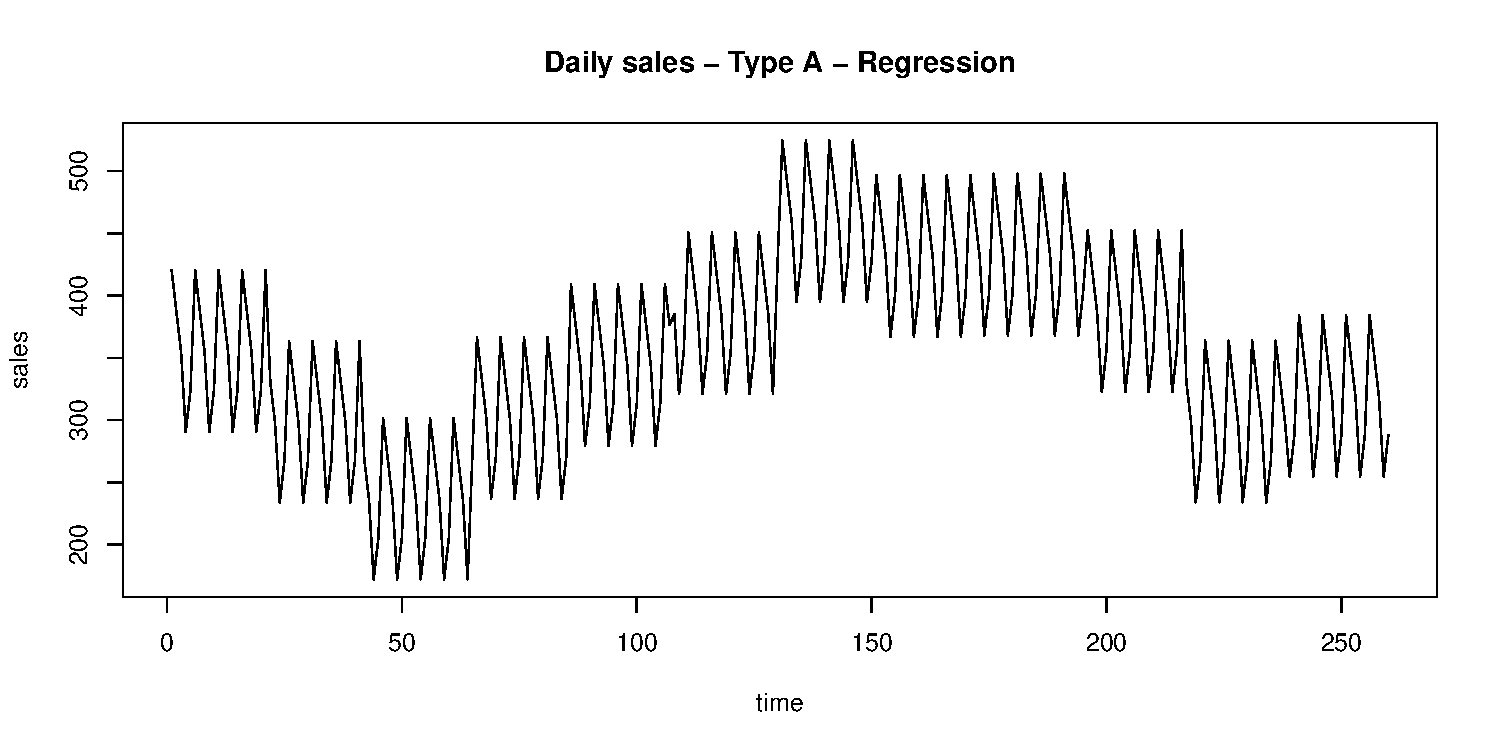
\includegraphics[width=\textwidth]{figures/fc_reg_A.pdf}
	\vskip -1.5em \caption{Regression - Tagesprognose - Kerzentyp A}
	\label{fig_reg_A}
\end{figure}

\begin{figure}[H]
	\centering
	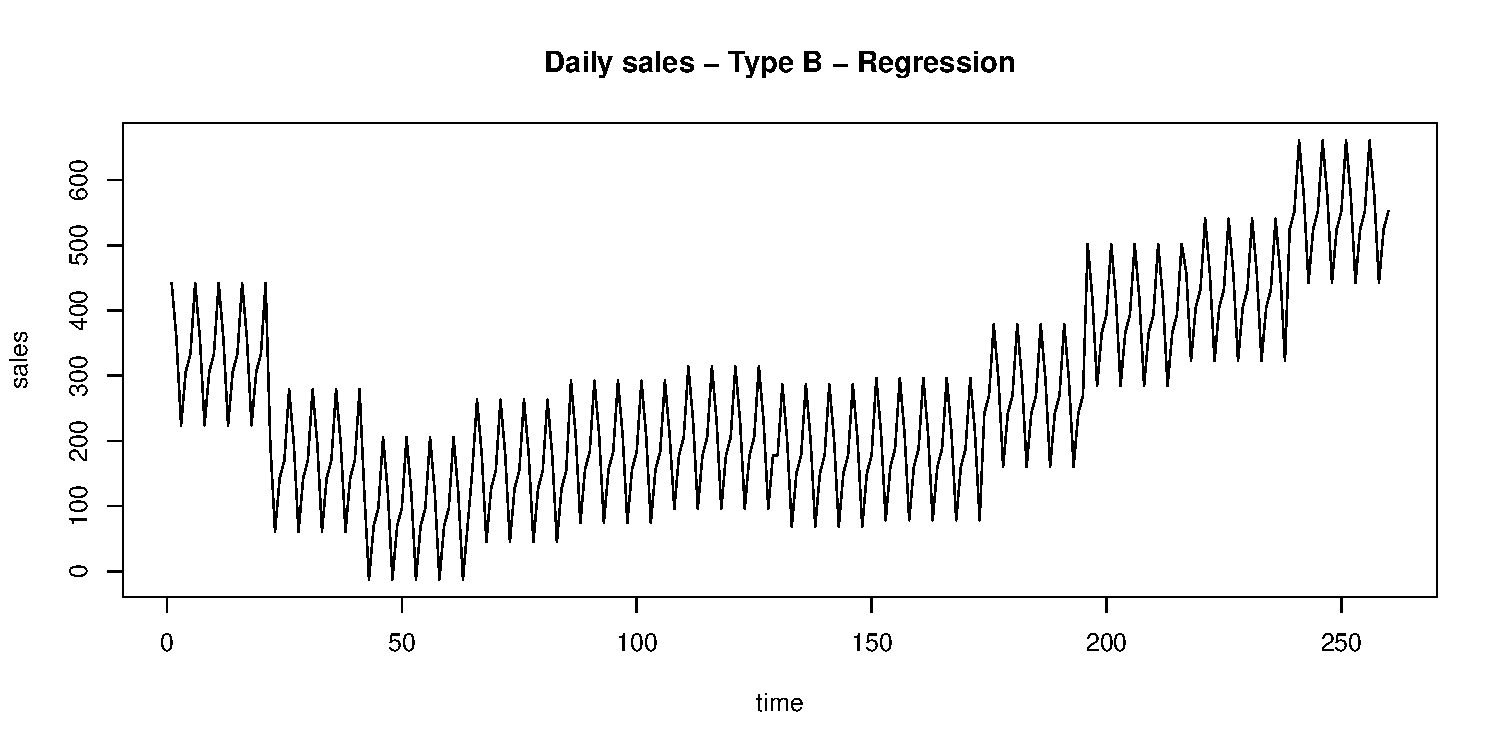
\includegraphics[width=\textwidth]{figures/fc_reg_B.pdf}
	\vskip -1.5em \caption{Regression - Tagesprognose - Kerzentyp B}
	\label{fig_reg_B}
\end{figure}

\begin{figure}[H]
	\centering
	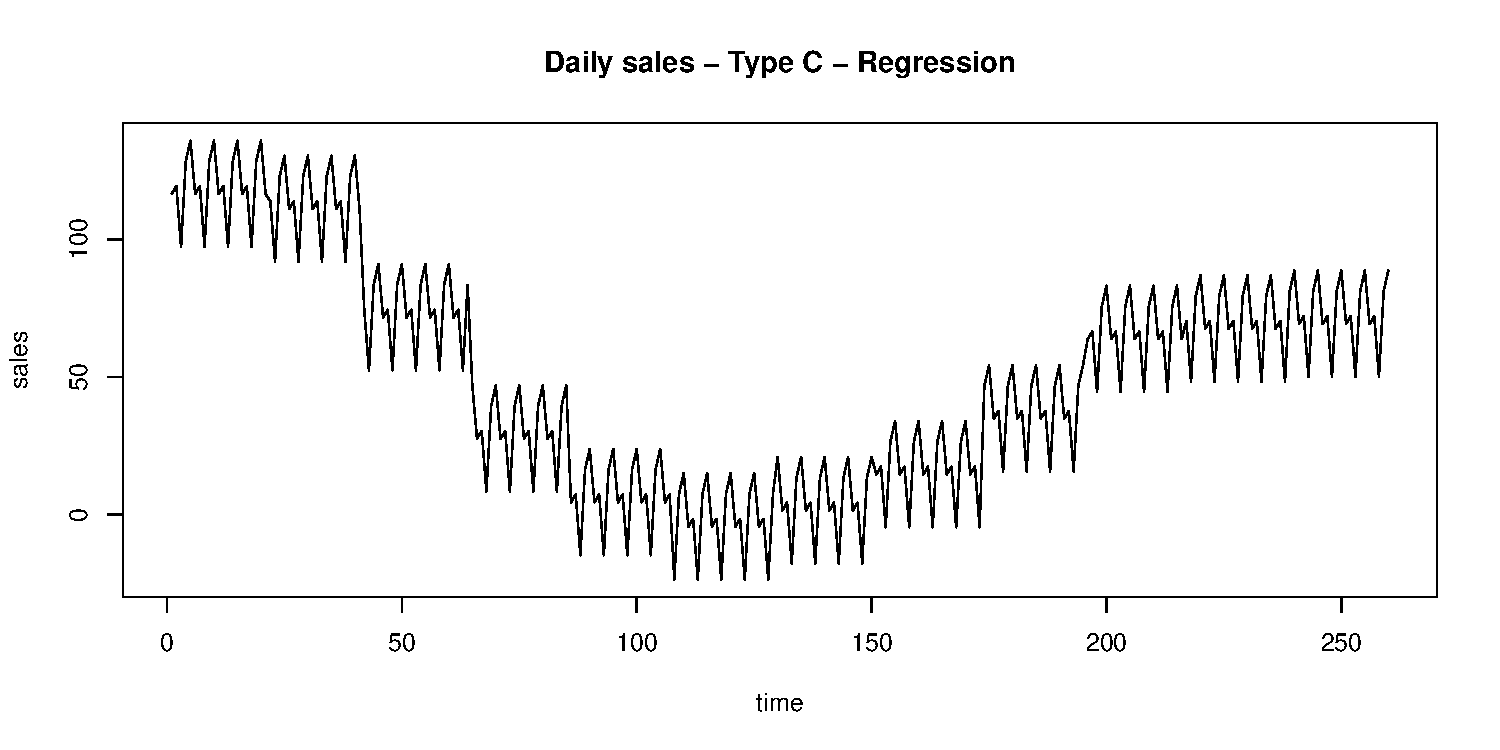
\includegraphics[width=\textwidth]{figures/fc_reg_C.pdf}
	\vskip -1.5em \caption{Regression - Tagesprognose - Kerzentyp C}
	\label{fig_reg_C}
\end{figure}

Die kumulierten Absätze ergeben uns einen "Fahrplan" der einzelnen Jahresabsätze der Produkte für das kommende Jahr.

\begin{figure}[H]
	\centering
	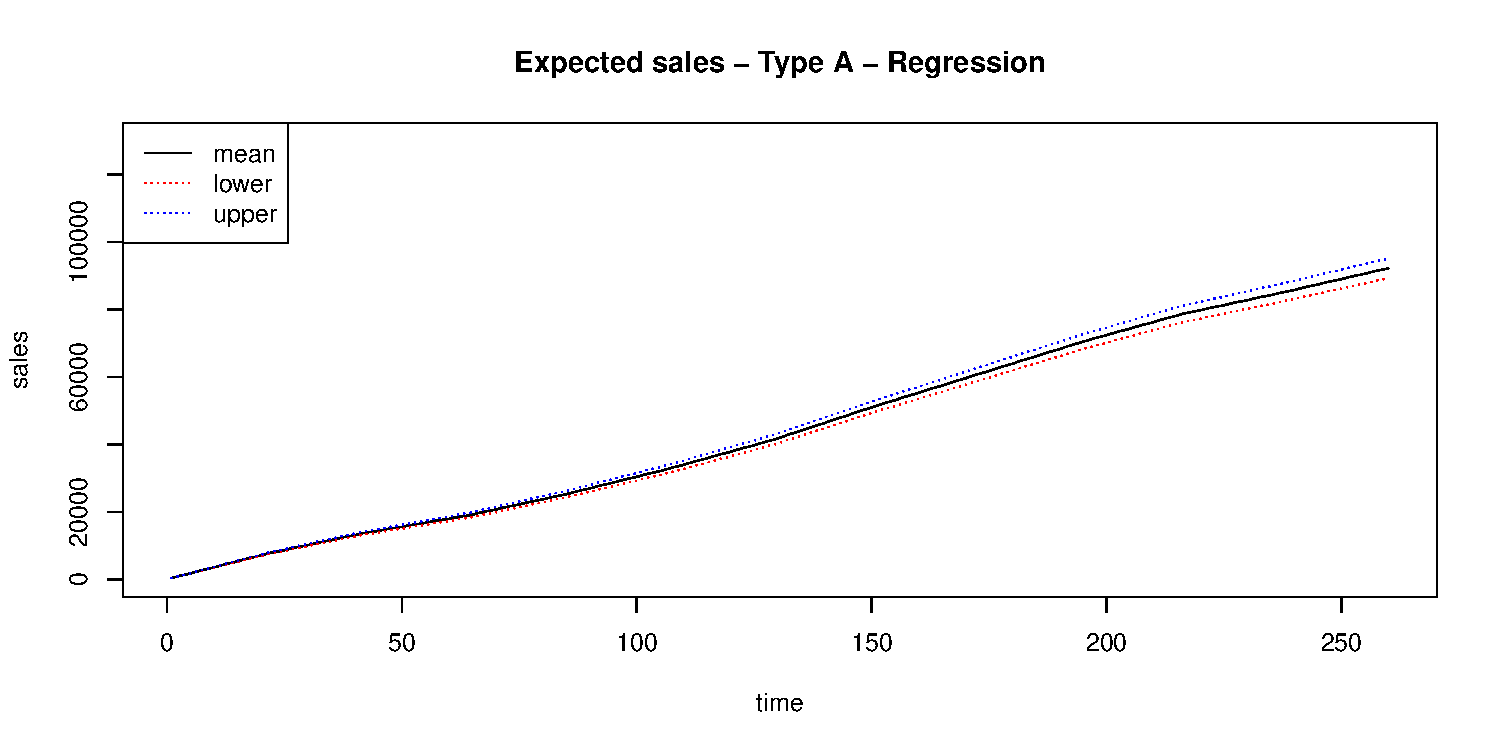
\includegraphics[width=\textwidth]{figures/traj_reg_A.pdf}
	\vskip -1.5em \caption{Regression - Jahresprognose - Kerzentyp A}
	\label{traj_reg_A}
\end{figure}

\begin{figure}[H]
	\centering
	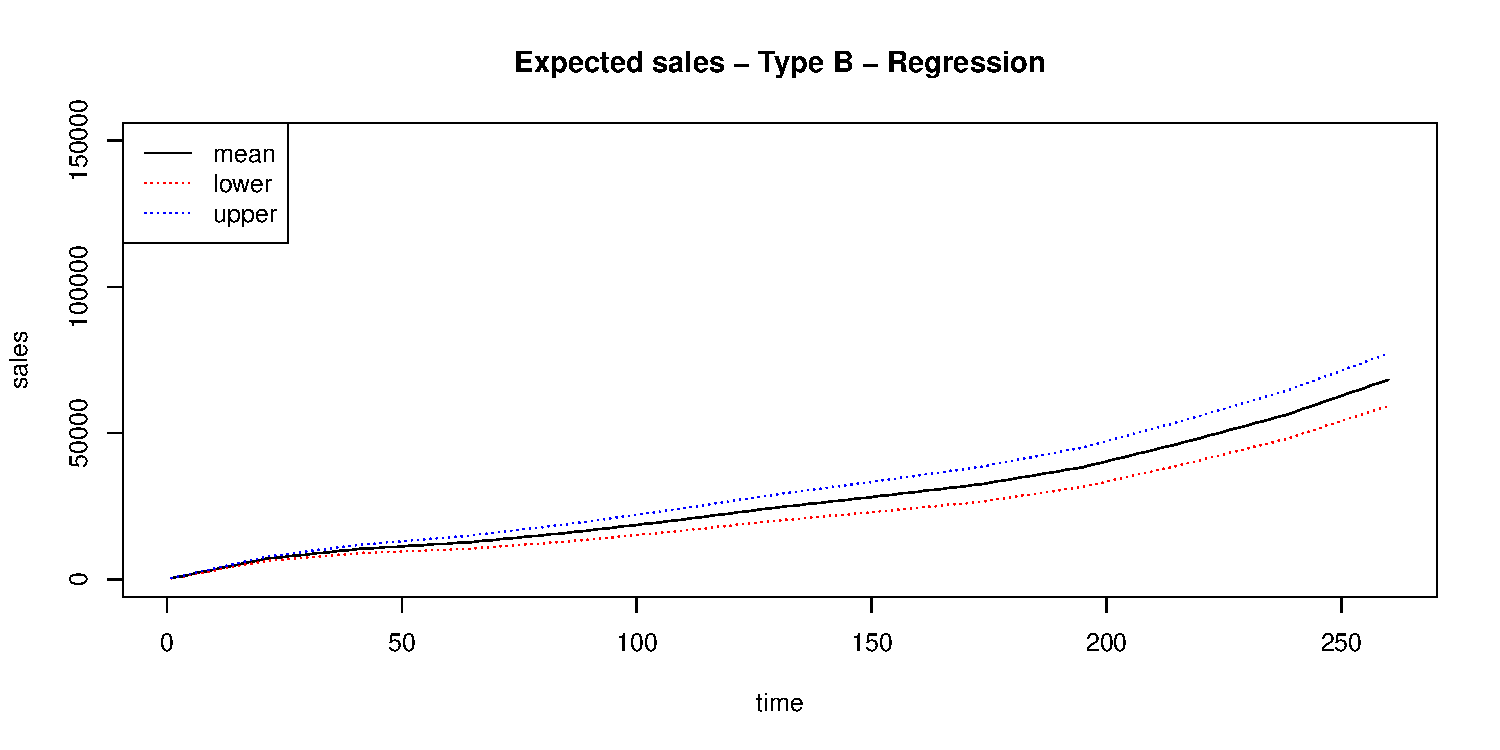
\includegraphics[width=\textwidth]{figures/traj_reg_B.pdf}
	\vskip -1.5em \caption{Regression - Jahresprognose - Kerzentyp B}
	\label{traj_reg_B}
\end{figure}

\begin{figure}[H]
	\centering
	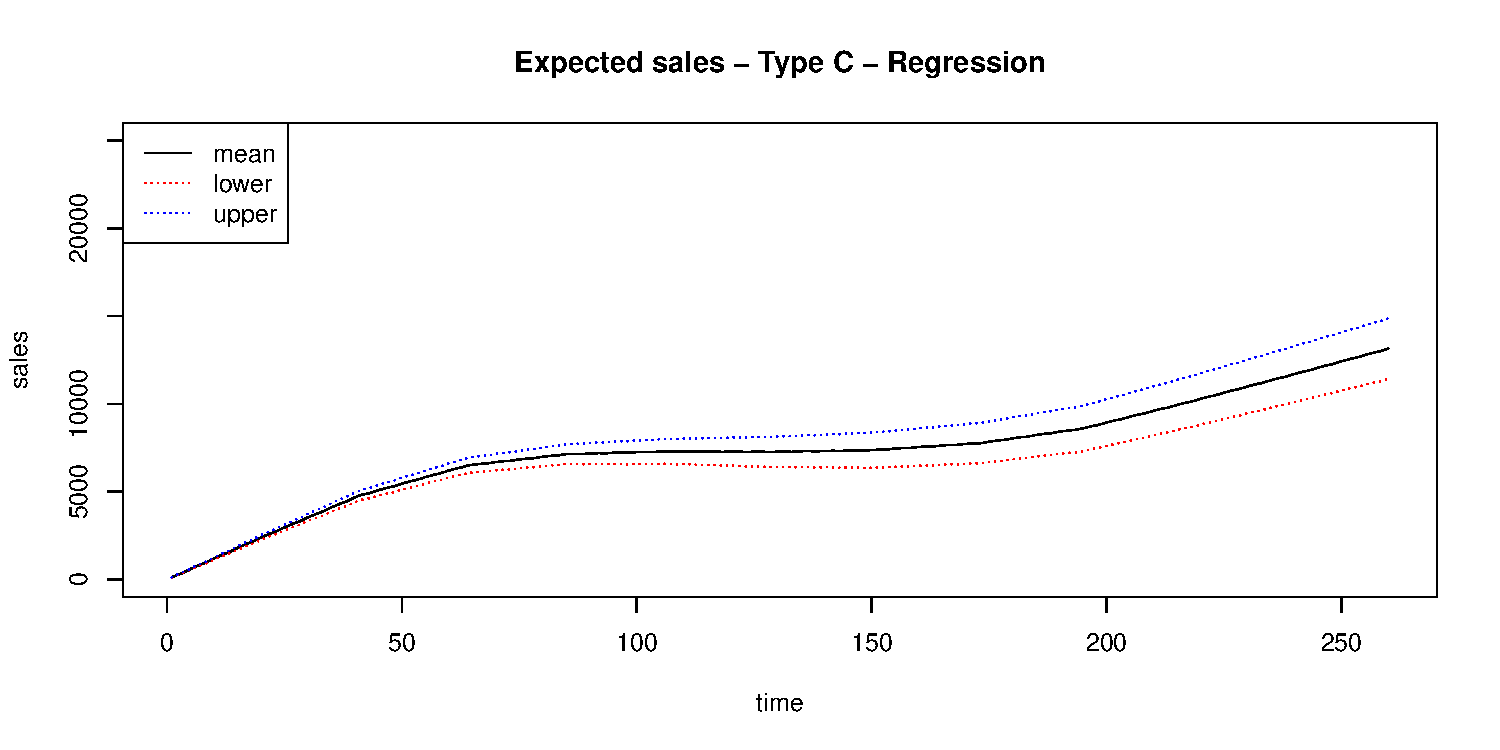
\includegraphics[width=\textwidth]{figures/traj_reg_C.pdf}
	\vskip -1.5em \caption{Regression - Jahresprognose - Kerzentyp C}
	\label{traj_reg_C}
\end{figure}

\newpage
\subsection{Angabe des R-Codes mit Erläuterungen}

\begin{lstlisting}
# Build some basic linear regression models
model.reg.A <- lm(A ~ year + as.factor(quarter) + as.factor(month) +
                      as.factor(dayOfWeek), data=candles.xts)
model.reg.B <- lm(B ~ year + as.factor(quarter) + as.factor(month) +
                      as.factor(dayOfWeek), data=candles.xts)
model.reg.C <- lm(C ~ year + as.factor(quarter) + as.factor(month) +
                      as.factor(dayOfWeek), data=candles.xts)

# Plot the residuals
plot(residuals(model.reg.A))
plot(residuals(model.reg.B))
plot(residuals(model.reg.C))

# Print the summary of all models
summary(model.reg.A)
summary(model.reg.B)
summary(model.reg.C)

# Build a planning period (= input data) to forecast on
forecast.reg.xts <- as.xts(seq(as.Date("2022-01-01"), as.Date("2022-12-31"),by='day'))
# Extract the needed additional variables
forecast.reg.xts$year       <- 3  # we "trust" the simple, linear trend
forecast.reg.xts$quarter    <- as.factor(quarters(index(forecast.reg.xts)))
forecast.reg.xts$month      <- as.factor(format(index(forecast.reg.xts), "%m"))
forecast.reg.xts$dayOfWeek  <- as.factor(format(index(forecast.reg.xts), "%u"))

# Exlude saturdays and sundays (since we got no sales there)
forecast.reg.xts <- subset(forecast.reg.xts, !(forecast.reg.xts$dayOfWeek %in% c(6,7)))

# Predict the upcoming year, including a 95% CI
forecast.reg.A <- predict(model.reg.A, forecast.reg.xts,
                          interval="confidence", level=0.95)
forecast.reg.B <- predict(model.reg.B, forecast.reg.xts,
                          interval="confidence", level=0.95)
forecast.reg.C <- predict(model.reg.C, forecast.reg.xts,
                          interval="confidence", level=0.95)

# Plot the basic forecasts
plot(forecast.reg.A[,"fit"], type='l')
plot(forecast.reg.B[,"fit"], type='l')
plot(forecast.reg.C[,"fit"], type='l')

# Convert them into dataframes for better plotting
forecast.reg.agg.A <- predict2dataframe(forecast.reg.A, TRUE)
forecast.reg.agg.B <- predict2dataframe(forecast.reg.B, TRUE)
forecast.reg.agg.C <- predict2dataframe(forecast.reg.C, TRUE)

# Plot the trajectories through the predicted year
cumsumplot(forecast.reg.agg.A, "Expected sales - Type A - Regression", scale.A)
cumsumplot(forecast.reg.agg.B, "Expected sales - Type B - Regression", scale.B)
cumsumplot(forecast.reg.agg.C, "Expected sales - Type C - Regression", scale.C)

# Plot the accumulated trajectory through the year (all candle sales)
ccumsumplot(forecast.reg.agg.A, forecast.reg.agg.B, forecast.reg.agg.C,
            "Expected sales - All candles - Regression", scale.ABC)
\end{lstlisting}

\newpage
\section{Quartalsweise Absatzzahlen: Stochastische prozessbasierte Budgetierung}

\subsection{Beschreibung der Vorgehensweise}

Um eine Vorhersage aufgrund eines stochastischen Gauß-Prozesses zu konstruieren (dieser betrachtet vor allem erwartete Absätze und Volatilitäten) ist es wichtig, eine Zeitperiode zu konstruieren die nicht "zu genau" ist. Eine Berechnung auf Tagesbasis würde eine zu große Ungenauigkeit beinhalten (da nur zwei gleiche Tage bekannt sind) - wir skalieren daher "hinunter" auf quartalsweise Daten. Außerdem kombinieren wir die einzelnen Absatzzahlen und erstellen unsere Prognose nur für die Absatzsumme A+B+C.\\

\begin{figure}[H]
	\centering
	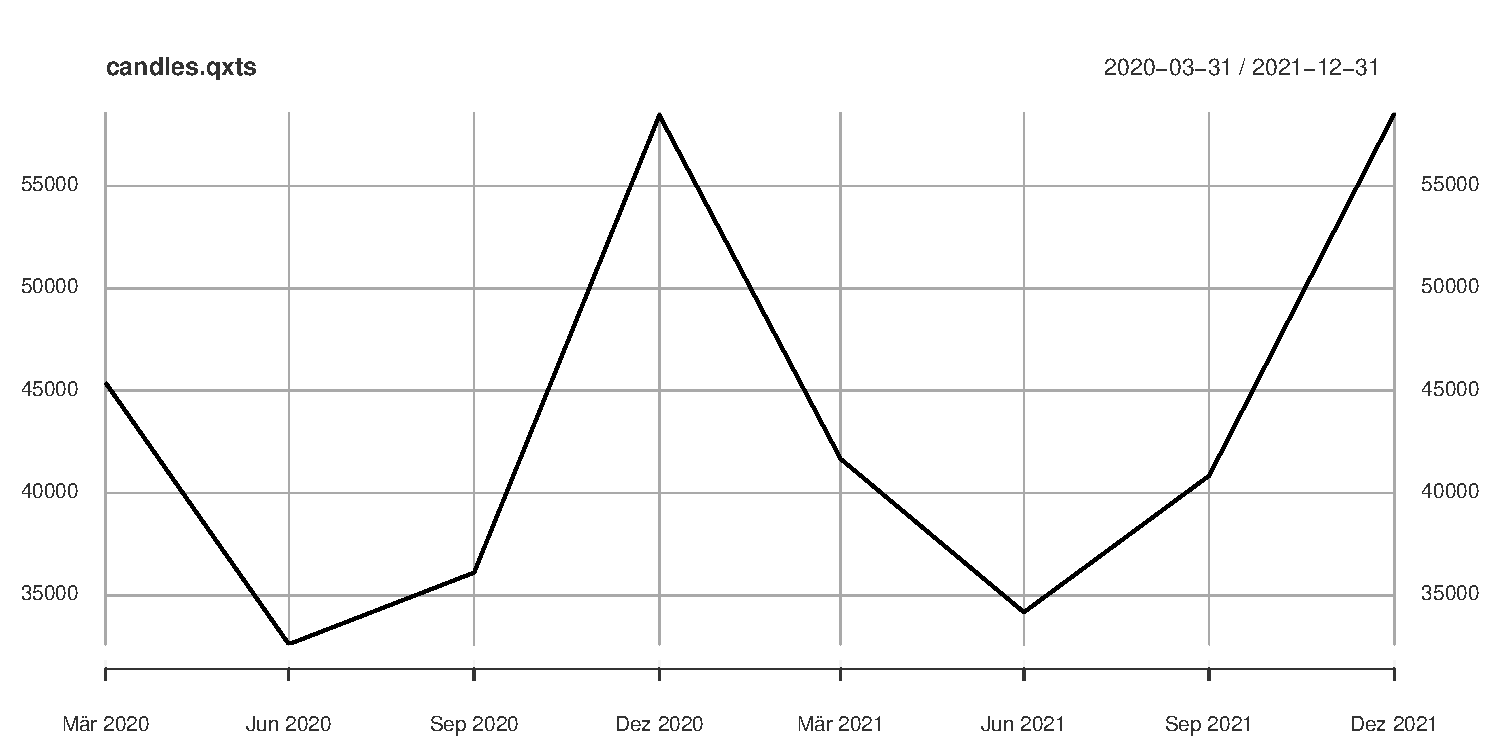
\includegraphics[width=\textwidth]{figures/quarterly.pdf}
	\vskip -1.5em \caption{Quartalsweise Absatzzahlen}
	\label{quarterly}
\end{figure}

Nun können wir für jedes Quartal die Erwartungswerte und Standardabweichungen der Absätze berechnen (hier ist zu beachten, dass "Standardabweichung" und "Erwartungswert" in unserer Form nur sinnvolle Aussagen sind, wenn wir davon ausgehen, dass sich unsere Absätze annähernd normalverteilt realisieren). Eine wichtige Kennzahl, die wir zusätzlich berechnen ist der sogenannten "Coefficient of Variation" (Variationskoeffizient):

\begin{equation}
	c_{\rm {v}}={\frac {\sigma }{\mu }},
\end{equation}

wobei $\mu$ und $\sigma$ den Erwartungswert bzw. die Standardabweichung bezeichnen. Der Variationskoeffizient ist eine statistische Kenngröße in der deskriptiven Statistik und der mathematischen Statistik. Im Gegensatz zur Varianz ist er ein relatives Streuungsmaß, das heißt, er hängt nicht von der Maßeinheit der statistischen Variable bzw. Zufallsvariable ab. Der Variationskoeffizient ist eine Normierung der Varianz: Ist die Standardabweichung größer als der Mittelwert bzw. der Erwartungswert, so ist der Variationskoeffizient größer 1.\\

Analysieren wir die Daten nämlich vor der Auswertung, so bemerken wir eine extrem kleine Varianz der Absätze in manchen Quartalen. Würden wir diese Information bestehen lassen, so würden wir für die Zukunft nicht mit einem normalverteilten Absatz planen (der sich unterschiedlich realisieren kann), sondern mit einer beinahe nicht-stochastischen Konstanten. Dies ist unwahrscheinlich, aufgrund der Tatsache, dass ein exakt gleicher Absatz im Folge Jahr äußerst unwahrscheinlich ist.\\

Um dieses Problem zu umgehen, fixieren wir den Variationskoeffizienten auf einen fixen minimalen Wert (in unserem Fall 5\%) und nutzen diesen - im Fall des Falles - zur Berechnung einer künstlichen Standardabweichung.\\

Nach Vorbereitung all dieser Kenndaten, können wir die Dichtefunktion der einzelnen Quartale (siehe \ref{density}) angeben sowie eine kumulierte Jahrestrajektorie (mit streuenden Unsicherheitsbändern die wir mittels der korrigierten Standardabweichung berechnen können) ausgeben.

\subsection{Mathematische Beschreibung der verwendeten Prognosemodelle}
\subsection{Erläuterung der Ergebnisse für gegossene, gezogene und gepresste Kerzen}

Wie bereits beschrieben, können wir mittels der gewonnenen Informationen die Dichtefunktionen der einzelnen Quartale darstellen (hier bereits mit Korrektur auf mind. 5\%-igen Variationskoeffizienten):

\begin{figure}[H]
	\centering
	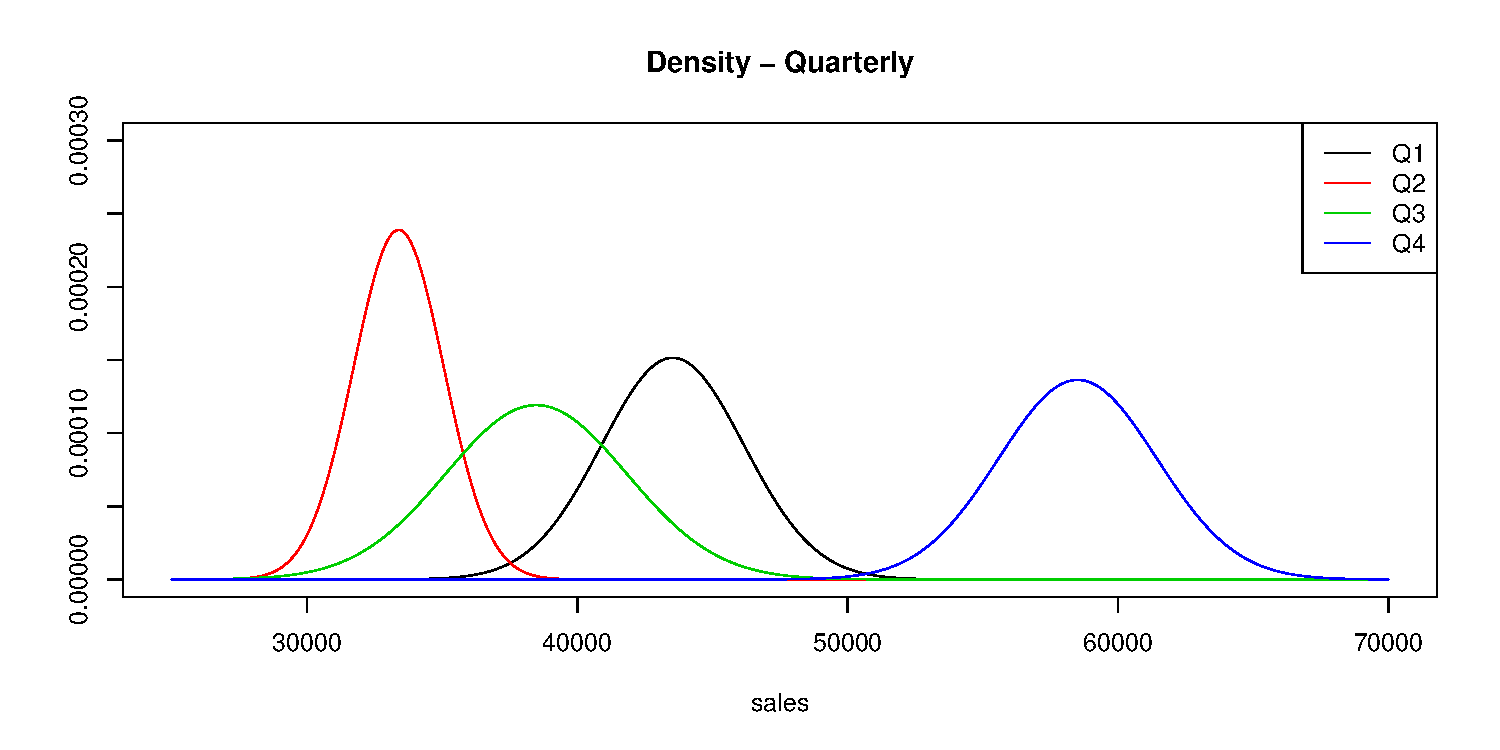
\includegraphics[width=\textwidth]{figures/density.pdf}
	\vskip -1.5em \caption{Dichtefunktion der Quartale 1-4 (A+B+C)}
	\label{density}
\end{figure}

Die "Sales at Risk" ergeben sich dann wie folgt:

\begin{figure}[H]
	\centering
	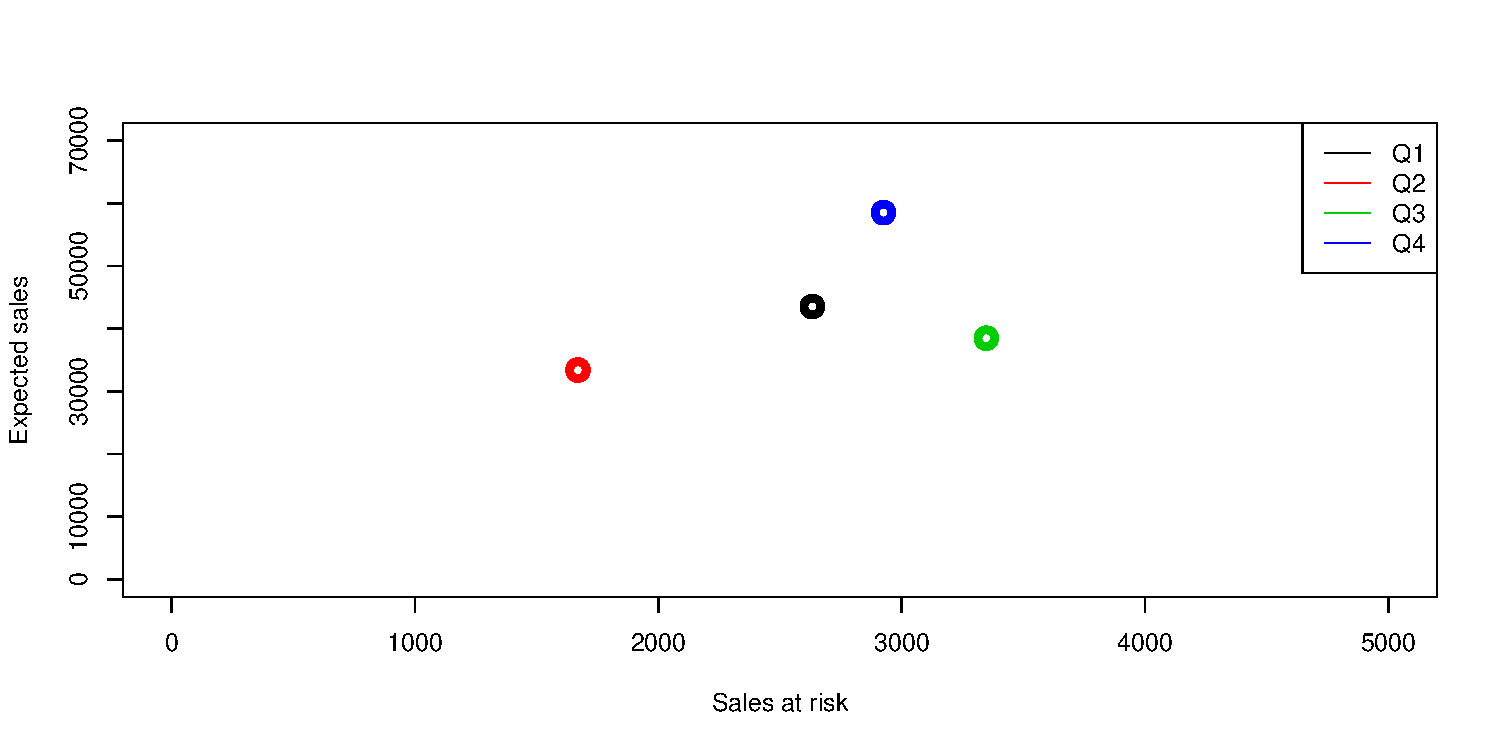
\includegraphics[width=\textwidth]{figures/salesatrisk.pdf}
	\vskip -1.5em \caption{"Sales at risk" der Quartale 1-4 (A+B+C)}
	\label{salesatrisk}
\end{figure}

Der Jahresabsatz sieht dann (in Dichte bzw. Wahrscheinlichkeit) so aus:

\begin{figure}[H]
	\centering
	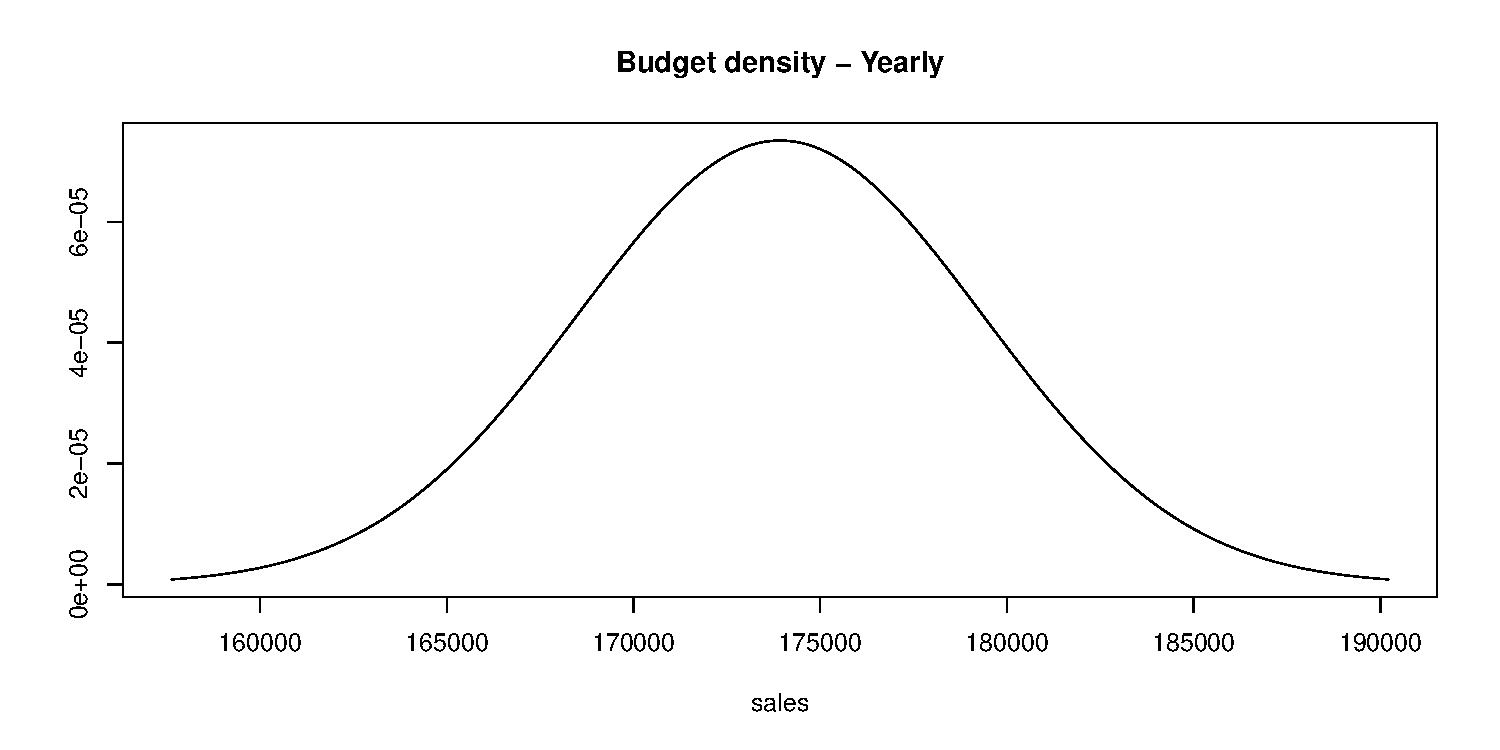
\includegraphics[width=\textwidth]{figures/stoch_dens.pdf}
	\vskip -1.5em \caption{Dichtefunktion des Jahresabsatzes (A+B+C)}
	\label{year_density}
\end{figure}

\begin{figure}[H]
	\centering
	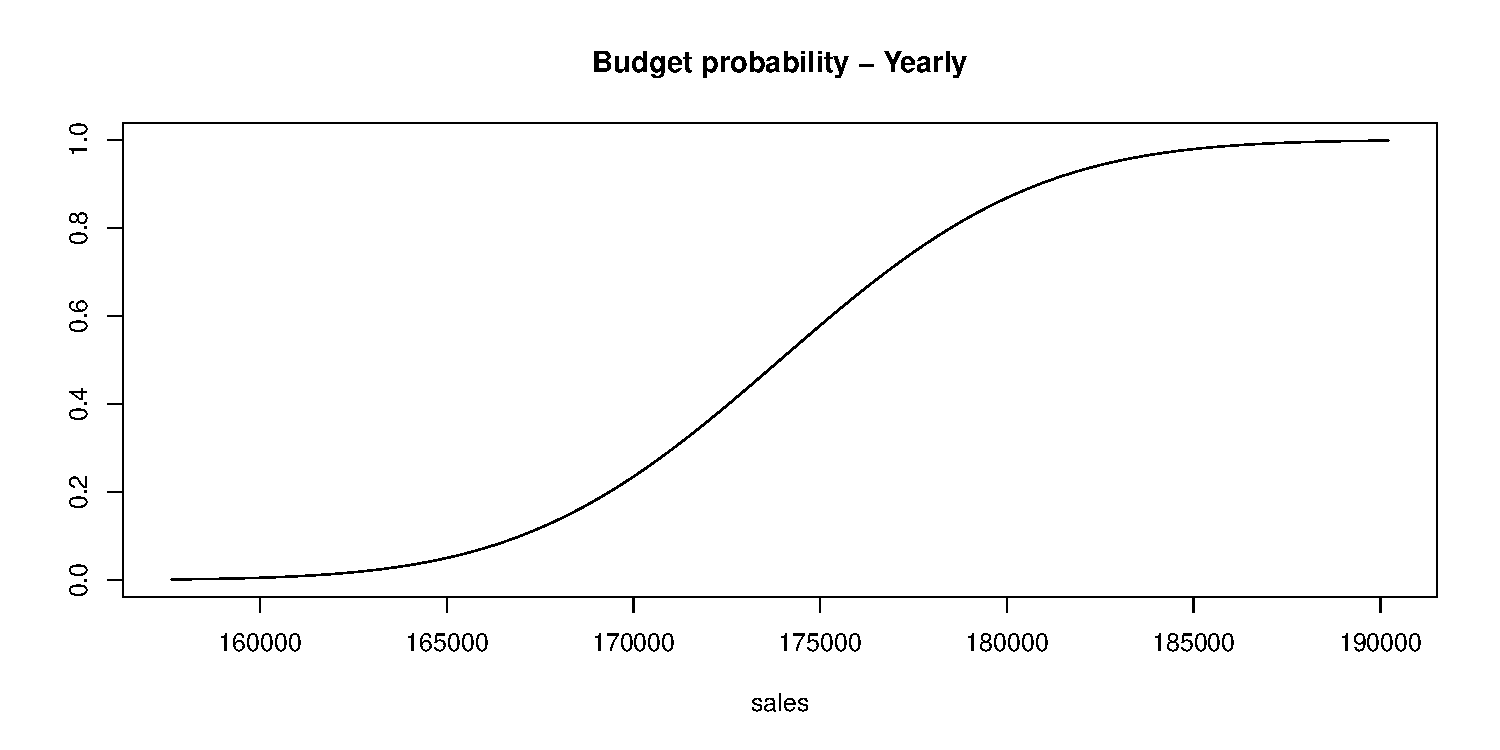
\includegraphics[width=\textwidth]{figures/stoch_prob.pdf}
	\vskip -1.5em \caption{Wahrscheinlichkeitsfunktion des Jahresabsatzes (A+B+C)}
	\label{year_prob}
\end{figure}

Die Jahresabsatztrajektorie (analog zu den anderen Prognosemodellen) sieht dann wie folgt aus:

\begin{figure}[H]
	\centering
	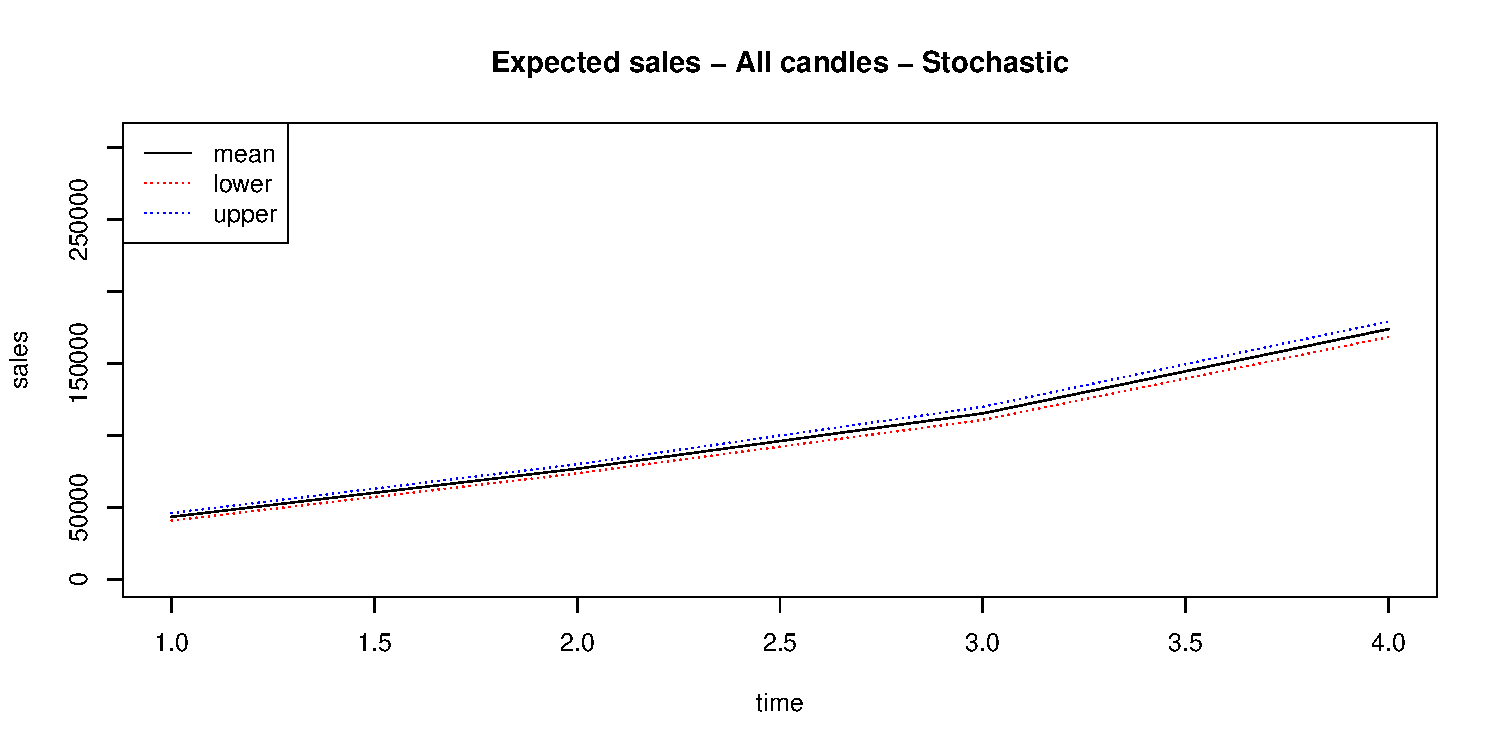
\includegraphics[width=\textwidth]{figures/fc_stoch_ABC.pdf}
	\vskip -1.5em \caption{Stochastischer Prozess - Jahresprognose - (A+B+C)}
	\label{year_traj}
\end{figure}

\subsection{Angabe des R-Codes mit Erläuterungen}

\begin{lstlisting}
# Extract the quarterly data and plot the trajectory through the given two years
candles.qxts <- apply.quarterly(candles.xts, sum)
colnames(candles.qxts) <- c("ABC")
plot(candles.qxts)

# Set up the used matrices
model.stoch.E  <- matrix(0, 1, 4)   # expected value
model.stoch.SD <- matrix(0, 1, 4)   # standard deviation
model.stoch.CV <- matrix(0, 1, 4)   # coefficient of variation

# Apply a min coefficient of variation. Why?
# We expect sales to vary by atleast X%. Sales staying the exact same over the
# course of several years can happen, but is extremely unlikely to happen again
minCV <- 0.05
# Set up the used matrices
model.stoch.SD.corr <- matrix(0, 1, 4)
model.stoch.CV.corr <- matrix(0, 1, 4)


# Apply readable column names
dimnames(model.stoch.E) <- list("ABC", c("Q1","Q2","Q3","Q4"))
dimnames(model.stoch.SD) <- list("ABC", c("Q1","Q2","Q3","Q4"))
dimnames(model.stoch.CV) <- list("ABC", c("Q1","Q2","Q3","Q4"))
dimnames(model.stoch.SD.corr) <- list("ABC", c("Q1","Q2","Q3","Q4"))
dimnames(model.stoch.CV.corr) <- list("ABC", c("Q1","Q2","Q3","Q4"))

# Calculate expected value, standard deviation and CV for every quarter
for (q in 1:4) {
model.stoch.E[1,q]  <- mean(candles.qxts[c(q,q+4),])
model.stoch.SD[1,q] <- sd(candles.qxts[c(q,q+4),])
model.stoch.CV[1,q] <- model.stoch.SD[1,q] / model.stoch.E[1,q]
}

# Correct the CV and SD by using the given min CV
model.stoch.CV.corr <- model.stoch.CV
model.stoch.CV.corr[model.stoch.CV.corr < minCV] <- minCV
model.stoch.SD.corr <- model.stoch.CV.corr * model.stoch.E

# Density plots of every quarter
sales <- 25000:70000
plot(sales,  dnorm(sales, model.stoch.E[1], model.stoch.SD.corr[1]),
     col=1, type="l", ylim=c(0,0.0003), ylab="", main="Density - Quarterly")
lines(sales, dnorm(sales, model.stoch.E[2], model.stoch.SD.corr[2]), col=2)
lines(sales, dnorm(sales, model.stoch.E[3], model.stoch.SD.corr[3]), col=3)
lines(sales, dnorm(sales, model.stoch.E[4], model.stoch.SD.corr[4]), col=4)
legend("topright", legend=c("Q1","Q2","Q3","Q4"), col=1:4, lty=1)

# Sales at risk (expected sales over volatility) of every quarter
plot(x=model.stoch.SD.corr, y=model.stoch.E, col=1:4, xlab="Sales at risk",
     ylab="Expected sales", xlim=c(0,5000), ylim=c(0,70000), cex=1.5, lwd=5)
legend("topright", legend=c("Q1","Q2","Q3","Q4"), col=1:4, lty=1)

# Plot the "stochastic" budget
yearE   <- cumsum(model.stoch.E)[4]
yearVol <- sqrt(cumsum((model.stoch.SD.corr)^2))[4]
plot(x=seq(yearE-3*yearVol,yearE+3*yearVol), y=pnorm(q=seq(yearE-3*yearVol,yearE+3*yearVol), mean=yearE, sd=yearVol), type="l", ylab="", xlab="sales", main="Budget probability - Yearly")
plot(x=seq(yearE-3*yearVol,yearE+3*yearVol), y=dnorm(x=seq(yearE-3*yearVol,yearE+3*yearVol), mean=yearE, sd=yearVol), type="l", ylab="", xlab="sales", main="Budget density - Yearly")

# Prepare a data.frame for trajectory plotting
forecast.stoch <- data.frame(
	cumsum(model.stoch.E),
	cumsum(model.stoch.E) - sqrt(cumsum((model.stoch.SD.corr)^2)),
	cumsum(model.stoch.E) + sqrt(cumsum((model.stoch.SD.corr)^2))
)
colnames(forecast.stoch) <- c("mean", "lower", "upper")
forecast.stoch$time <- 1:4

# Plot the accumulated trajectory through the year (all candle sales)
cumsumplot(forecast.stoch, "Expected sales - All candles - Stochastic", scale.ABC)
\end{lstlisting}

\newpage
\section{Zusammenfassung und Ausblick}
Zuerst betrachten wir die prognostizierten Jahresabsätze der einzelnen Algorithmen (jeweils gemeinsam mit einem 95\% CI). Wir sehen, dass sowohl die Regression als auch die Stochastische Planung einen erwarteten Absatz von rund 173000 Stück ergeben. Dieser Wert wird durch die zeitreihenbasierte Vorhersage etwas höher geschätzt: 185000. Auch die Unsicherheit ist hier (aufgrund der "fehler-kumulierenden" Wirkung der zugrunde liegenden ARMA Struktur) höher.
\begin{lstlisting}
"------- STL + ETS -------"
"Mean:   185613"
"Lower:  139253"
"Upper:  231974"

"------- Regression -------"
"Mean:   173714"
"Lower:  165776"
"Upper:  181652"

"------- Stochastic -------"
"Mean:   173924"
"Lower:  168493"
"Upper:  179355"
\end{lstlisting}

\vskip 3em

Um die Aussage der drei unterschiedlichen Prognosen über den (erwarteten) Jahresabsatz besser verstehen zu können, stellen wir die drei Trajektorien in einer Grafik dar: 

\begin{figure}[H]
	\centering
	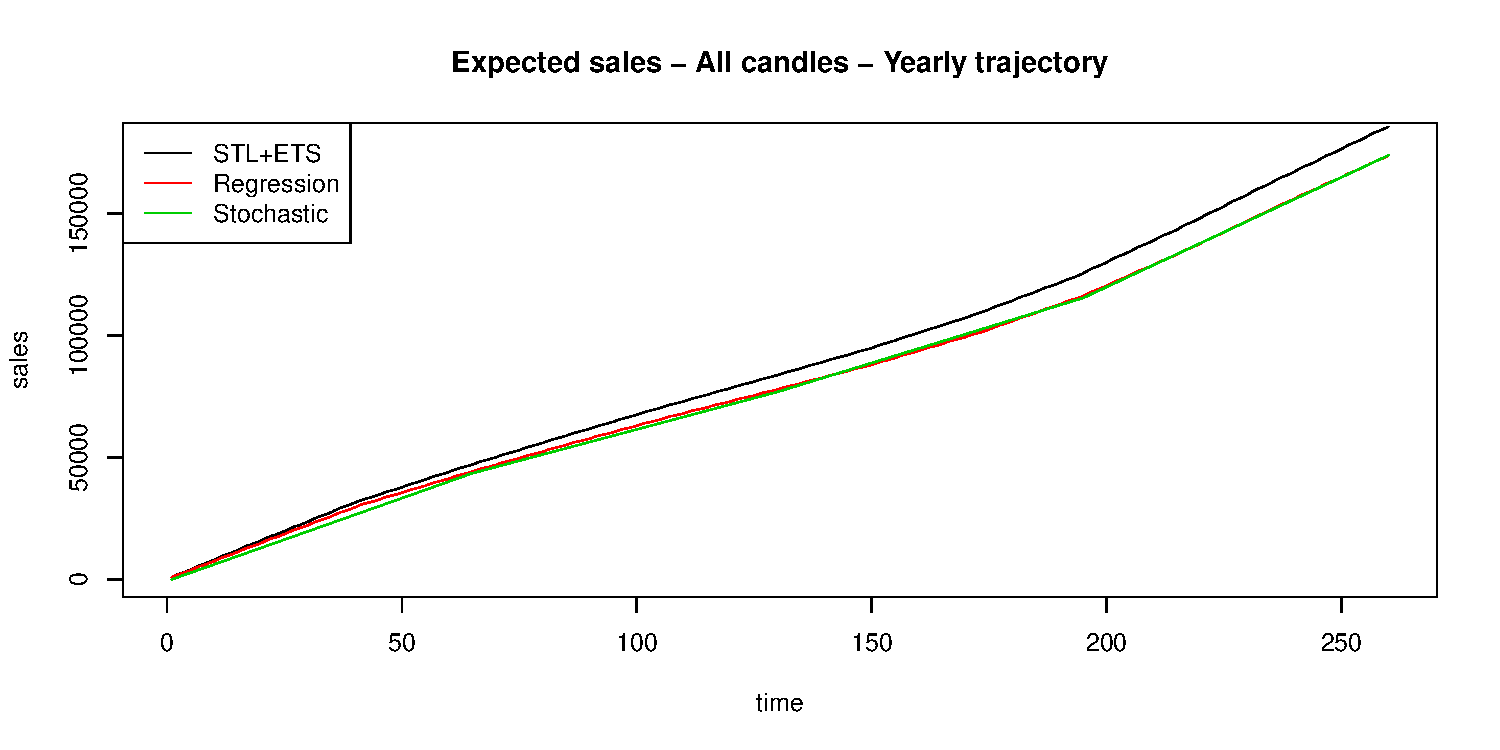
\includegraphics[width=\textwidth]{figures/traj_all.pdf}
	\vskip -1.5em \caption{Vergleich aller Prognose-Algorithmen für die jährliche Absatzsumme A+B+C}
	\label{traj_all}
\end{figure}

Diese Grafik unterlegt die oben bereits angeführten numerischen Ergebnisse. Der Unterschied besteht größtenteils darin, dass die zeitreihenbasierte Prognose einen geringeren Abwärtstrend der Verkäufe im nächsten Jahr sieht - der prinzipielle Verlauf ist jedoch beinahe ident.\\

\newpage
Grundlegend lassen sich folgende Charakteristiken über die gezeigten Prognoseverfahren zusammenfassen:

\begin{itemize}
	\item Zeitreihen: Sind grundsätzlich sehr gut geeignet, wenn aufgrund bereits realisierter Absätze eine Prognose $n$ Tage in die Zukunft durchgeführt werden soll. Hierfür kann der Algorithmus tagesaktuell mit neuen Daten neu gestartet werden und das Resultat ausgewertet werden. Interessiert man sich für erklärbare Daten oder für eine speziell Prognose (z.B. "Absatz am zweiten Dienstag im Monat Juli") ist die Aussagekraft beschränkt und die Unsicherheit hoch.
	\item Regression: Bietet den großen Vorteil, erklärende Daten zu liefern. So können Einflüsse von Wochentagen, Feiertagen, Quartalen und vielen anderen erklärenden Variablen untersucht werden (z.B. könnte man die Absätze auch auf andere erzeugbare Daten regressieren; wie Wetter, Sonnenstunden, ...). Zu beachten ist - wie bei vielen anderen Algorithmen auch, aber hier besonders - dass die Qualität der Aussage stark von der Parametrisierung (hier vor allem Wahl des Regressionsmodells sowie der erklärenden Variablen abhängt). Overfitting oder die Wahl eines unnötig komplizierten Regressionsalgorithmus (z.B.: ist ein Tobit-Modell wirklich notwendig/ sind die Daten wirklich zensiert?) können die Aussagekraft stark verfälschen.
	\item Stochastischer Prozess: Bietet den großen Vorteil einer "konkreten" Angabe in welchem Bereich sich mit welcher Wahrscheinlichkeit die Absatzzahlen bewegen. Die Frage "Wird der Absatz im Intervall $[a,b]$ liegen?", ist für vorgegebenes Intervall schnell und anschaulich beantwortbar. Welche Anpassungen, grundlegende Daten, Frequenzen der Auswertung und ähnliches untersucht werden, liegt jedoch allein im Auge des Betrachters - ist also stark von menschlichen Subjektivitäten abhängig.
\end{itemize}

Daraus ergibt sich folgende Empfehlung zur Implementierung:
\begin{itemize}
	\item Ein zeitreihenbasiertes Modell zur tagesaktuellen Vorhersage kurzfristiger Absätze.
	\item Ein regressionsbasiertes Modell zur Untersuchung und Erklärung des Kunden-/Kaufverhaltens.
	\item Ein stochastisches Modell zur einfachen Untersuchung und Planung verschiedener vorgegebener Budgetpläne von Seiten der GF.
\end{itemize}


\newpage
\bibliographystyle{plain}
\bibliography{bib}



\end{document}